\documentclass[12pt]{report}

\usepackage[utf8]{vietnam}
\usepackage{graphicx}
\usepackage{svg}
\usepackage{fancyhdr}
\usepackage{parskip}
\usepackage{amssymb}
\usepackage{amsmath}
\usepackage{float}
\usepackage{tikz}
\usepackage{fancybox}
\usetikzlibrary{positioning}
\usepackage[left=3 cm,right=3 cm,top=3cm,bottom=3cm]{geometry}
\usepackage[labelfont=bf]{caption}
\usepackage[unicode]{hyperref}
\usepackage{bookmark}
\usepackage{enumitem}
\usepackage[bottom]{footmisc}
\usepackage{multirow}

\pagestyle{fancy}
\fancyhf{}
\fancyhead[R]{\normalsize{\textit{\leftmark}}}
\fancyhead[LE,LO]{\thepage}
\renewcommand{\headrulewidth}{0.4pt}

\graphicspath{{images/}}

%-----------------SET PARAMS----------------------------------
\tikzset{
  treenode/.style = {shape=rectangle,
                     draw, align=center,
                     top color=white, bottom color=blue!20},
  root/.style     = {treenode, font=\Large, bottom color=red!30},
  env/.style      = {treenode, font=\ttfamily\normalsize},
  dummy/.style    = {circle,draw}
}
%---------------END OF SET PARAMS---------------------------

\begin{document}

%---------------SET FOR DIAGRAM------------------------------
\usetikzlibrary{arrows,chains,positioning,scopes}

\tikzset{
    block/.style={draw,thick,text width=5em,minimum height=6.5em,minimum width=5em,align=center},
    arrow/.style={->, thick}
}

%------------------TITLE PAGE-----------------------------------
\begin{titlepage}

\newcommand{\HRule}{\rule{\linewidth}{0.5mm}} % Defines a new command for the horizontal lines, change thickness here

\center % Center everything on the page
 
%----------------------------------------------------------------------------------------
%	HEADING SECTIONS
%----------------------------------------------------------------------------------------
\begin{flushright}
\end{flushright}
\textsc{\large ĐẠI HỌC BÁCH KHOA THÀNH PHỐ HỒ CHÍ MINH}\\[0.2cm]
\textsc{\Large \scshape khoa khoa học và kỹ thuật máy tính}\\[0.5cm]
\begin{figure}[H] 
\centering

\includegraphics[scale=1.6]{images/logo.jpg}
\end{figure} 

\textsc{\large LUẬN VĂN TỐT NGHIỆP}\\[0.2cm] % Minor heading such as course title

%----------------------------------------------------------------------------------------
%	TITLE SECTION
%----------------------------------------------------------------------------------------
\HRule \\[0.4cm]
{ \huge \bfseries Phân giải đồng tham chiếu \\ cho đối tượng và thuộc tính \\ trong khai khoáng ý kiến}\\[0.4cm] % Title of your document
\HRule \\[0.8cm]

%----------------------------------------------------------------------------------------
%	AUTHOR SECTION
%----------------------------------------------------------------------------------------
\begin{flushright}
\begin{minipage}{0.7\textwidth}

\end{minipage}
\end{flushright}

\begin{flushleft} \large
\textbf{Giáo viên hướng dẫn:}\\
GS. TS. Phan Thị Tươi\\[2.0cm]
\end{flushleft}

\begin{flushleft} \large
\textbf{Sinh viên thực hiện:}\\
Nguyễn Đăng Trang - 51203957\\
Nguyễn Trọng Nghĩa - 51202370\\[2cm]
\end{flushleft}

\begin{flushleft} \large
\centering
TP. Hồ Chí Minh, tháng 12 năm 2016
\end{flushleft}

\vfill % Fill the rest of the page with whitespace

\end{titlepage}
%----------------END TITLE PAGE--------------------

\newpage
	\chapter*{Lời cam đoan}
		\par Chúng tôi xin cam đoan rằng, tất cả mọi kết quả được thể hiện trong Luận văn, ngoại trừ những kết quả được trích dẫn nguồn rõ ràng, đều do chính chúng tôi thực hiện.

		\begin{flushright}
			TP. Hồ Chí Minh, ngày 16 tháng 12 năm 2016
		\end{flushright}

\newpage
	\chapter*{Lời cảm ơn}
		\par Trước tiên, chúng tôi xin gửi lời cảm ơn sâu sắc tới cô giáo GS.TS Phan Thị Tươi, người đã luôn theo sát hướng dẫn và giúp đỡ tận tình chúng tôi trong suốt quá trình thực hiện Luận văn để chúng tôi hoàn thành đề tài Luận văn của mình. Bên cạnh đó chúng tôi cũng muốn gửi lời cảm ơn chân thành tới các thầy cô của Khoa Khoa học và kỹ thuật máy tính - trường Đại học Bách Khoa TP. Hồ Chí Minh, những kiến thức mà họ truyền đạt thực sự là những hành trang hữu ích mà chúng tôi có được trong suốt những năm tháng học đại học. Cuối cùng, chúng tôi xin được gửi lời tri ân tới gia đình và bạn bè, những người đã luôn ủng hộ chúng tôi về mặt tinh thần để chúng tôi có được những kết quả ngày hôm nay. 

		\begin{flushright}
			Nhóm tác giả
		\end{flushright}

\newpage
	\thispagestyle{empty}
	\pdfbookmark{\contentsname}{Mục lục}
	\tableofcontents
	\pagenumbering{arabic}

\newpage
  	\addcontentsline{toc}{chapter}{Danh sách hình vẽ}
	\listoffigures
	\addcontentsline{toc}{chapter}{Danh sách bảng}
	\listoftables

\newpage
	\chapter{Tóm tắt Luận văn}		
		\par Ngôn ngữ của con người chứa đựng nhiều đặc trưng phức tạp và làm cách nào để cho máy tính khai phá có hiệu quả loại dữ liệu này vẫn là một vấn đề lớn. Khai khoáng ý kiến là một lĩnh vực mới phát triển gần đây của Xử lý ngôn ngữ tự nhiên và đang ngày càng có những ứng dụng rộng rãi, nó hướng đến việc tìm ra những ý kiến, cảm xúc được biểu đạt qua ngôn ngữ. Bên cạnh đó, bài toán phân giải đồng tham chiếu, mặc dù đã được nghiên cứu rộng rãi nhưng vẫn chỉ được thực hiện trên các loại văn bản chung chung. Các văn bản chứa ý kiến như các bài đánh giá (review), các thảo luận (discussion) về các sản phẩm với các đặc trưng riêng của nó, cung cấp thêm những thông tin nhất định cho việc phân giải đồng tham chiếu trên đó có hiệu quả hơn. 
		\par Trong Luận văn này, chúng tôi đề xuất bài toán \textit{Phân giải đồng tham chiếu cho đối tượng và thuộc tính trong Khai khoáng ý kiến} với cách tiếp cận theo mô hình \textit{Học có giám sát}. Mục tiêu của bài toán là tìm xem những từ/cụm từ nào trong văn bản cùng chỉ về đối tượng hoặc thuộc tính. Dữ liệu được dùng là các văn bản chứa ý kiến bằng ngôn ngữ tiếng Anh. Mô hình do chúng tôi đề xuất cho kết quả khả quan và gợi mở ra những hướng đi cho việc thực hiện Phân giải đồng tham chiếu cho các văn bản chứa ý kiến trong tiếng Việt.
		\par Luận văn được tổ chức thành 6 chương. Chương 2 nêu ra vấn đề và giới thiệu về đề tài \textit{Phân giải đồng tham chiếu cho đối tượng và thuộc tính trong Khai khoáng ý kiến}, chương này cũng đồng thời nói về phạm vi và mục đích của đề tài. Chương 3 là các kiến thức nền tảng được sử dụng trong việc thực hiện đề tài, đó là các nội dung về bài toán Phân giải đồng tham chiếu, Khai khoáng ý kiến và giải thuật học máy Cây quyết định. Chương 4 nói về Phương pháp đề xuất và cách hiện thực hệ thống giải quyết bài toán đặt ra. Trong chương 5, các kết quả thực nghiệm và các đánh giá, phân tích của chúng tôi được dẫn ra. Cuối cùng, chúng tôi tổng kết lại Luận văn của mình trong chương cuối - chương 6.
		
	\chapter{Giới thiệu đề tài}	
		\label{introduction_chapter}
		\par \textit{Phân giải đồng tham chiếu (Coreference resolution)} là một bài toán quan trọng và được nghiên cứu rộng rãi trong Xử lý ngôn ngữ tự nhiên \cite{mainpaper}. Mục tiêu của bài toán là tìm ra trong văn bản những đề cập (mention) cùng chỉ về một (tập) thực thể trong thế giới thực và gom nhóm chúng thành các chuỗi đồng tham chiếu.\\
		Ví dụ: \\
		"\textit{Beckham} will visit Vietnam tomorrow. \textit{He} will attend a football event in Saigon."\\
		\textit{Beckham} và \textit{he} trong ví dụ trên cùng chỉ về một thực thể (con người) là cầu thủ bóng đá David Beckham, chúng đồng tham chiếu với nhau.
		\par Tuy nhiên, những nghiên cứu hiện tại về bài toán đồng tham chiếu mới chỉ dừng lại trên các nội dung văn bản tổng quát và không tập trung vào một loại văn bản cụ thể nào. Mặt khác, cùng với sự phát triển nhanh chóng của thương mại điện tử, người dùng ngày càng có nhu cầu thể hiện ý kiến, cảm xúc của mình đối với sản phẩm. Điều đó được thể hiện qua các bài đánh giá (review) khi mua sắm sản phẩm trực tuyến, các bài đăng (blog post), hay các bài thảo luận trên diễn đàn về sản phẩm (discussion). Trong các văn bản này, người dùng đánh giá về các sản phẩm, cụ thể là họ thể hiện ý kiến đối với đối tượng sản phẩm (object) và các thuộc tính (attribute) của sản phẩm. 
		\par Đối tượng (object) là các thực thể có tên chỉ sản phẩm, mỗi đối tượng bao gồm một tập các bộ phận (component) và một tập các tính chất (feature). Mỗi bộ phận cũng có một tập các bộ phận con và một tập các tính chất của nó. Nói một cách tổng quát, đối tượng có thể được biểu diễn bởi một cây mà nút (node) gốc chính là đối tượng và các nút con là các bộ phận, mối liên kết giữa các nút là các quan hệ thành phần (part-of) \cite{sentiment}. Khi thể hiện ý kiến, người dùng hướng ý kiến đến các nút của cây và các tính chất của các nút.\\
		Ví dụ:\\
		"\textit{The Samsung Galaxy S3} is one of the best phones I've ever used. I absolutely love the phone and \textit{the photo quality} \underline{it} has".\\
		Trong ví dụ trên, người dùng đang đánh giá về đối tượng là chiếc điện thoại \textit{The Samsung Galaxy S3} và thuộc tính của nó là \textit{the photo quality}. Rõ ràng nếu không có phân giải đồng tham chiếu cho đại từ \textit{it}, chúng ta không biết được \textit{it} đang chỉ tới thực thể gì, là đối tượng \textit{The Samsung Galaxy S3} hay thuộc tính \textit{the photo quality}.
		\par Hơn nữa, nếu không có phân giải đồng tham chiếu, một lượng thông tin về ý kiến có thể bị mất đi.\\
		Ví dụ:\\
		"The Galaxy III is pretty cool (1). It's a plastic phone, but it feels solid even though it's very light (2). The screen looks great (3). It is very sharp (4)".
		\\Chúng ta có thể biết được người dùng thể hiện ý kiến ở câu (2) và (4). Nhưng nếu không có phép phân giải đồng tham chiếu để xác định các đại từ "it" trong câu (2) cùng chỉ về đối tượng "The Galaxy III" trong câu (1) và "It" trong câu (4) chỉ về thuộc tính "The screen" trong câu (3), chúng ta không thể biết được người dùng đang thể hiện ý kiến trên thực thể nào.
		\par Trong các văn bản có chứa ý kiến, ngoài đối tượng được xác định là các thực thể có tên, thuộc tính được giả định là đã được tìm ra. Hu và Liu (2004) trong \cite{findfeatures1}, Popescu và Etzionie (2005) trong \cite{findfeatures2} đã trích xuất ra tập thuộc tính gắn với đối tượng (mà họ gọi là \textit{features}). Nhiệm vụ của đề tài là tìm xem những từ/cụm từ nào cùng chỉ về đối tượng hoặc thuộc tính.

	\chapter{Các công trình liên quan}				
		\section{Các công trình liên quan đến phân giải đồng tham chiếu nói chung}
			\par Phân giải đồng tham chiếu là một chủ đề quan trọng trong Xứ lý ngôn ngữ tự nhiên, nó ảnh hưởng đến kết quả của các chủ đề khác như: trích xuất thông tin (information extraction), hỏi đáp tự động (question answering), tóm tắt văn bản (text summarization),... Vì vậy đã có rất nhiều công trình làm về chủ đề này. Căn cứ vào hướng tiếp cận bài toán đồng tham chiếu, chúng tôi chia các công trình liên quan thành 3 nhóm: Mô hình cặp, mô hình thực thể, mô hình xếp hạng. Căn cứ vào giải thuật được áp dụng vào bài toán đồng tham chiếu hay nói cách khác là cách sử dụng tập dữ liệu, các công trình liên quan thành 3 nhóm: Học có giám sát (supervised learning), học không giám sát (unsupervised learning), hệ thống luật (rules-system).
			Thống nhất một vài khái niệm, kí hiệu:
				\begin{itemize}
					\item{Yêu cầu của bài toán đồng tham chiếu: Tìm tất cả các chuỗi đồng tham chiếu trong một văn bản; trong đó, mỗi chuỗi đồng tham chiếu là tập hợp các cụm danh từ cùng chỉ đến một thực thể trong thực tế. Từ yêu cầu bài toán, ta thấy đây là một bài toán gom cụm.} 
					\item{Chúng tôi sử dụng khái niệm "cặp" để nói đến cặp gồm hai cụm danh từ. Kí hiệu cặp (NP1, NP2) được hiểu gồm cụm danh từ NP1 và NP2. Trong đó NP1 xuất hiện trước NP2 trong văn bản, NP1 được gọi là tiền từ và NP2 được gọi là hậu từ.}
					\item{Hai cụm danh từ cùng chỉ đến một thực thể là đồng tham chiếu với nhau và chúng nằm trong cùng một chuỗi đồng tham chiếu. Cặp đồng tham chiếu nếu hai cụm danh từ của cặp đồng tham chiếu với nhau và cặp không đồng tham chiếu nếu hai cụm danh từ không đồng tham chiếu.}
					\item{Kí hiệu NPs thể hiện tập hợp chứa nhiều hơn 1 cụm danh từ}
				\end{itemize}
			\par \textit{Căn cứ theo cách tiếp cận bài toán đồng tham chiếu, các công trình liên quan được chia làm 3 nhóm được trình bày dưới đây, gồm: mô hình cặp, mô hình thực thể và mô hình xếp hạng}
			\subsection*{Mô hình cặp (Mention pair)}
				\par Ý tưởng:  Xác định các cặp đồng tham chiếu, sau đó kết hợp các cặp đồng tham chiếu tìm được thành chuối đồng tham chiếu. Bài toán trở thành bài toán phân loại, phân loại tích cực nếu cặp đồng tham chiếu và tiêu cực nếu cặp không đồng tham chiếu.
				\begin{figure}[H]
					\centering
					% Author: Rasmus Pank Roulund
% \documentclass{minimal}
% \usepackage{tikz}
% \usepackage[utf8]{vietnam}

% \begin{document}
% \usetikzlibrary{arrows,chains,positioning,scopes}

\tikzset{
    block/.style={draw,thick,text width=5em,minimum height=6.5em,minimum width=5em,align=center},
    arrow/.style={->, thick}
}
\begin{tikzpicture}
  {[start chain]
      \node[block,on chain] (N1) {Tập hợp các cụm danh từ};
      \node[block,on chain,join=by {arrow},right=1cm of N1] (N2) {Tạo tập các cặp cụm danh từ};
      \node[block,on chain,join=by {arrow},right=1cm of N2] (N3) {Phân loại các cặp cụm danh từ};
      \node[block,on chain,join=by {arrow},right=1cm of N3] (N4) {Kết hợp những cặp được phân loại đồng tham chiếu};
      \node[block,on chain,join=by {arrow},right=1cm of N4] (N5) {Các chuỗi đồng tham chiếu};
    }
      
  \end{tikzpicture}
% \end{document}
					\caption{Ý tưởng các bước thực hiện trong Mô hình cặp}
				\end{figure}
				\par Theo như mô hình trình bày ý tưởng từ hình vẽ, mỗi tác giả sẽ có một cách riêng khi thực hiện các bước:
				\begin{itemize}
					\item{Tạo tập các cặp.}
					\item{Tạo tập thuộc tính để phân loại một cặp là đồng tham chiếu hay không.}
					\item{Cách kết hợp kết quả từ các cặp thu được để tạo ra chuỗi đồng tham chiếu.}
				\end{itemize}
				\par Dưới đây chúng tôi trình bày chi tiết về 2 bước là: Cách tạo tập thuộc tính và cách kết hợp kết quả từ các cặp.
				\begin{itemize}
					\item{Tạo tập thuộc tính: 
						\\Để xác định cặp có đồng tham chiếu hay không, ta cần phải dựa vào tập thuộc tính được tạo ra từ 2 NPs của cặp đó. Tập thuộc tính được tạo ra từ đặc điểm cấu trúc cú pháp, ngữ pháp, ngữ nghĩa. Những thuộc tính cơ bản về cú pháp và ngữ nghĩa được trình bày rõ ràng trong bài báo của Ng và Cardie (2002)\cite{ng02}. Theo thời gian, thuộc tính cú pháp không còn gì để bổ sung thêm nên những công trình sau này chủ yếu đề xuất thêm những thuộc tính về ngữ nghĩa, ví dụ: Dagan và Itai (1990)\cite{dagan90}; Kehler (2004)\cite{kehler04}; Yang (2005)\cite{yang05}; Haghighi và Klein (2009)\cite{haghighi09}.}
					\item{Cách kết hợp kết quả từ các cặp: 
						\\Từ kết quả xác định đồng tham chiếu của mỗi cặp NPs, tính chất bắc cầu được sử dụng để tạo các chuỗi đồng tham chiếu. Ví dụ: nếu A đồng tham chiếu B, B đồng tham chiếu C $\rightarrow$ Cụm đồng tham chiếu {A B C} gồm A, B và C. Tuy nhiên, trước khi áp dụng tính chất bắc cầu, cần phải có giải thuật để lựa chọn lại các cặp NPs đã được phân loại tích cực. Một số giải thuật được sử dụng phổ biến để đáp ứng yêu cầu đó là:
						\begin{itemize}
							\item{Giải thuật gom cụm gần nhất (closest-first clustering) được đề xuất bởi Soon (2001)\cite{soon01}: Nếu có các cặp được dự đoán đồng tham chiếu mà hậu từ giống nhau thì Soon chỉ giữ lại cặp đồng tham chiếu mà có khoảng cách từ tiền từ đến hậu từ là gần nhất.}
							\item{Giải thuật gom cụm tốt nhất (best-first clustering) được sử dụng bởi Ng và Cardie (2002)\cite{ng02}: Nếu có các cặp được dự đoán đồng tham chiếu mà hậu từ giống nhau thì Ng chỉ giữ lại cặp đồng tham chiếu được dự đoán với trọng số (khả năng) cao nhất.}
							\item{Giải thuật gom cụm dựa trên đồ thị (graph partitioning algorithms) được nhắc đến bởi McCallum và Wellner (2004)\cite{mccallum04}: Gom cụm dựa trên đồ thị vô hướng có trọng số được xây dựng từ các cặp kết quả. Trong đó, mỗi đỉnh đại diện cho một cụm danh từ và mỗi cạnh có trọng số là giá trị phân loại của cặp hai NPs.}
						\end{itemize}}
						\par  Việc sử dụng tính chất bắc cầu để gom cụm có nhược điểm là: Những cặp có quyết định tích cực được thiên vị hơn những cặp có quyết định tiêu cực. Ví dụ: Mặc dù A và C rõ ràng là không đồng tham chiếu, nhưng nếu A và B đồng tham chiếu, B và C đồng tham chiếu thì A và C vẫn sẽ được quyết định là đồng tham chiếu.
				\end{itemize}			 
				\par Ưu điểm của mô hình cặp: Đơn giản, dễ hiện thực.
				\par Nhược điểm của mô hình cặp:
					\begin{itemize}
						\item{Bài toán được đề ra là bài toán gom cụm, tuy nhiên cách hiện thực lại là kết hợp phân loại trước, gom cụm sau. Kĩ thuật gom cụm ảnh hưởng đến kết quả. Mặc dù có thể cố gắng điều chỉnh kết quả ở bước phân loại, nhưng không ảnh hưởng đến kết quả cuối cùng.}
						\item{Để kiểm tra xem cặp 2 NPs có đồng tham chiếu không, tập thuộc tính chỉ được tạo ra dựa trên 2 NPs đó. Sẽ gặp những trường hợp có những thuộc tính không xác định được. Ví dụ: Trong câu \textit{"Mr.Clinton has a new phone. Clinton also has a new camera. He’s so rich"}, ta không thể xác định Clinton và He có cùng thuộc tính giới tính hay không. Trong trường hợp đó, nếu ta đã biết Mr.Clinton và Clinton đồng tham chiếu và sử dụng được thuộc tính giới tính từ Mr.Clinton, ta có thể suy ra Clinton và He có cùng thuộc tính giới tính.}
						\item{Đối với một NP. Ta sẽ xét các cặp từ NP với các tiền từ của nó. Mặc dù có thể dự đoán ra đồng tham chiếu, tuy nhiên ta không thể xác định tiền từ nào phù hợp nhất với một NP vì ta dự đoán độc lập cặp từng tiền từ với NP.}
					\end{itemize}
			\subsection*{Mô hình thực thể (Entity-mention)}
				\par Ý tưởng: Xác định xem một cụm danh từ có đồng tham chiếu với một chuỗi đồng tham chiếu (thực thể) hay không. Mục đích của mô hình là phân loại liệu cụm danh từ NP\textsubscript{$k$} và chuỗi đồng tham chiếu $C_{j}$ là tích cực hay tiêu cực, đồng nghĩa với NP\textsubscript{$k$} có nên được gán vào chuỗi $C_{j}$ không. Hình 2 trình bày các bước trong mô hình thực thể.
				\begin{figure}[H]
					\centering
					% Author: Rasmus Pank Roulund
% \documentclass{minimal}
% \usepackage{tikz}
% \usepackage[utf8]{vietnam}

% \begin{document}
% \usetikzlibrary{arrows,chains,positioning,scopes}

\tikzset{
    block/.style={draw,thick,text width=10em,minimum height=6.5em,minimum width=11em,align=center},
    arrow/.style={->, thick}
}
\begin{tikzpicture}
  {[start chain]
      \node[block,on chain] (N1) {Tập hợp các cụm danh từ};
      \node[block,on chain,join=by {arrow},right=1cm of N1] (N2) {Xem mỗi cụm danh từ là một chuỗi đồng tham chiếu};
      \node[block,on chain,join=by {arrow},right=1cm of N2] (N3) {Tạo các cặp chứa hai chuỗi đồng tham chiếu};
      \node[block,on chain,join=by {arrow},below=1cm of N3] (N4) {Phân loại các cặp đã tạo};
      \node[block,on chain,join=by {arrow},left=1cm of N4] (N5) {Nếu cặp nào được phân loại đồng tham chiếu, gộp hai chuỗi của cặp đó làm một};
      \node[block,on chain,join=by {arrow},left=1cm of N5] (N6) {Các chuỗi đồng tham chiếu};      
    }
      
  \end{tikzpicture}
% \end{document}
					\caption{Một hiện thực điển hình của mô hình thực thể}
				\end{figure}
				Mỗi cụm danh từ NP\textsubscript{$k$} và chuỗi đồng tham chiếu $C_{j}$ có một tập thuộc tính dùng để phân loại. Tập thuộc tính này gồm: các thuộc tính của NP\textsubscript{$k$}, các thuộc tính liên quan giữa NP\textsubscript{$k$} với $C_{j}$. Điểm đặc trưng của mô hình thực thể và cụm danh từ chính là tập thuộc tính liên quan giữa NP\textsubscript{$k$} với $C_{j}$. Để xác định một thuộc tính giữa NP\textsubscript{$k$} với $C_{j}$, ta xét thuộc tính đó giữa NP\textsubscript{$k$} với các cụm danh từ trong $C_{j}$, từ đó tổng hợp lại. Ví dụ: Để kiểm tra thuộc tính NUMBER AGREEMENT xem NP\textsubscript{$k$} có cùng ngôi với $C_{j}$ không, trước tiên ta kiểm tra lần lược NP\textsubscript{$k$} có cùng ngôi với các cụm danh từ trong $C_{j}$ không. Sau đó ta tổng hợp lại kết quả, một vài cách tổng hợp: NUMBER AGREEMENT là YES nếu NP\textsubscript{$k$} cùng ngôi với tất các các NPs trong $C_{j}$, NO trong trường hợp còn lại; hoặc như Lou (2004)\cite{lou04} hay Yang (2004, 2008)\cite{yang04}\cite{yang08}, NUMBER AGREEMENT là YES nếu NP\textsubscript{$k$} cùng ngôi với ít nhất một NP trong $C_{j}$, NO trong tường hợp còn lại.
				\par Có nhiều biến thể, hình thức hiện thực mô hình thực thể, song vẫn giữ nguyên nét đặc trưng là: xây dựng thuộc tính của chuỗi đồng tham chiếu dựa trên các cụm danh từ của nó. Cullota (2007)\cite{culotta07} giải quyết bài toán đồng tham chiếu bằng cách xác định xác suất một cụm chứa các NPs từ văn bản có phải là một chuỗi đồng tham chiếu. Để thực hiện mục tiêu đó, tác giả dựa vào thuộc tính chung của cụm NPs. Với thuộc tính X của cụm NPs, X nhận giá trị ALL nếu tất cả các cặp của cụm NPs cùng có thuộc tính X, X nhận giá trị MOST-TRUE nếu đa số các cặp của NPs có cùng thuộc tính X và X nhận giá trị MOST-FALSE nếu đa số các cặp của NPs không có cùng thuộc tính X. 
				\par Ưu điểm của mô hình thực thể: Khắc phục được nhược điểm của mô hình cặp (mention pair), đó là sử dụng thuộc tính của chuỗi đồng tham chiếu, các NPs trong chuỗi có thể bổ sung thuộc tính cho nhau. Tuy nhiên khi áp dụng vào thực tế thì kết quả của hệ thống đồng tham chiếu cũng không được cải thiện nhiều, theo Luo (2004)\cite{lou04}, Yang (2004, 2008)\cite{yang04}\cite{yang08}. Lí do mà các tác giả trên đưa ra là họ vẫn sử dụng ít thuộc tính của chuỗi đồng tham chiếu.
			\subsection*{Mô hình xếp hạng (Ranking mention)}
				\par Ý tưởng: Xét cụm danh từ NP, so sánh tất cả các cụm danh từ đứng trước NP với nhau, tìm xem cụm danh từ nào có khả năng đồng tham chiếu với NP nhất. Ta thấy ý tưởng cũng gần giống với mô hình cặp, đầu ra của cả hai mô hình là cặp đồng tham chiếu. Hình vẽ 3 trình bày ý tưởng các bước của mô hình.
				\begin{figure}[H]
					\centering
					% Author: Rasmus Pank Roulund
% \documentclass{minimal}
% \usepackage{tikz}
% \usepackage[utf8]{vietnam}

% \begin{document}
% \usetikzlibrary{arrows,chains,positioning,scopes}

\tikzset{
    block/.style={draw,thick,text width=6em,minimum height=10em,minimum width=7em,align=center},
    arrow/.style={->, thick}
}
\begin{tikzpicture}
  {[start chain]
      \node[block,on chain] (N1) {Tập hợp các cụm danh từ};
      \node[block,on chain,join=by {arrow},right=1cm of N1] (N2) {Lọc lại các cụm danh từ có khả năng nằm trong chuỗi đồng tham chiếu};
      \node[block,on chain,join=by {arrow},right=1cm of N2] (N3) {Với một cụm danh từ, so sánh các ứng viên cụm danh từ nằm bên trái của nó};
      \node[block,on chain,join=by {arrow},right=1cm of N3] (N4) {Lựa chọn ứng viên có khả năng đồng tham chiếu cao nhất};
      \node[block,on chain,join=by {arrow},below=1cm of N4] (N5) {Tạo các cặp cụm danh từ đồng tham chiếu};
      \node[block,on chain,join=by {arrow},left=1cm of N5] (N6) {Kết hợp những cặp đồng tham chiếu};
      \node[block,on chain,join=by {arrow},left=1cm of N6] (N7) {Tạo các chuỗi đồng tham chiếu};      
    }
      
  \end{tikzpicture}
% \end{document}
					\caption{Ý tưởng các bước của mô hình xếp hạng}
				\end{figure}
				\par Mô hình xếp hạng được áp dụng vào phân giải đồng tham chiếu lần đầu bởi Connolly (1994; 1997)\cite{connolly95}\cite{connolly97}. Cụm danh từ NP\textsubscript{$k$} có một Tập tiền ngữ chứa các tiền ngữ của nó. Xét các cặp (NP\textsubscript{$i$},NP\textsubscript{$j$},NP\textsubscript{$k$}) có thể trong đó NP\textsubscript{$i$} và NP\textsubscript{$j$} thuộc K, phân loại xem (NP\textsubscript{$i$},NP\textsubscript{$j$},NP\textsubscript{$k$}) là tích cực hay tiêu cực, nếu tích cực thì NP\textsubscript{$i$} đồng tham chiếu với NP\textsubscript{$k$}, nếu tiêu cực thì NP\textsubscript{$j$} dồng tham chiếu với NP\textsubscript{$k$}. Từ kết quả các cặp được xây dựng từ NP\textsubscript{$k$}, tiền từ nào có số lần phân loại đồng tham chiếu với NP\textsubscript{$k$} cao nhất thì tiền ngữ đó đồng tham chiếu với NP\textsubscript{$k$}.
				Một vài biến thể dưới tên gọi khác nhau của mô hình thực thể: mô hình cạnh tranh (tournament model) của tác giả Iida (2003)\cite{iida03} hay mô hình hai ứng viên (the twin-candidate model) được sử dụng bởi Yang (2003, 2008)\cite{yang03}\cite{yang08}. 
				\par Ưu điểm của mô hình xếp hạng: So sánh được giữa các tiền từ của một NP, xem tiền từ nào phù hợp đồng tham chiếu nhất. Nói cách khác, mô hình trả lời được câu hỏi tiền từ nào phù hợp đồng tham chiếu nhất với một hậu từ cho trước mà mô hình cặp không thể làm được.
				\par Nhược điểm của mô hình xếp hạng: Phải thực hiện tác vụ loại bỏ bớt các cụm danh từ NPs từ văn bản mà không có khả năng nằm trong chuỗi đồng tham chiếu. Bới vì những cụm danh từ được giữ lại chắc chắn sẽ được phân loại nằm trong một chuỗi đồng tham chiếu nào đó. Điều này ảnh hưởng đến độ chính xác (precision)  của mô hình. Denis và Baldridge (2008)\cite{denis08} và Rahman and Ng (2009)\cite{rahman09} đã đề xuất một vài phương pháp để giải quyết nhược điểm này.					
				\par Một số tác giả kết hợp các mô hình trong 3 mô hình trên lại với nhau, trong đó kể đến Rahman and Ng (2009)\cite{rahman09} kết hợp mô hình thực thể với sắp xếp, mục đích so sánh các chuỗi đồng tham chiếu xem chuỗi nào phù hợp với một cụm danh từ đang xét. Mô hình đã khắc phục được hai điểm yếu của mô hình mention pair và cải thiển được kết quả.
			\par \textit{Căn cứ theo giải thuật được sử dụng trong bài toán đồng tham chiếu, các công trình liên quan được chia làm 3 nhóm được trình bày dưới đây, gồm: Giải thuật học có giám sát, giải thuật học không giám sát và hệ thống luật}
				\subsection*{Giải thuật học có giám sát}
					\par Định nghĩa: Giải thuật học có giám sát là giải thuật sử dụng tập dữ liệu có gán nhãn (đã biết trước kết quả) để học. Hai nhánh giải thuật lớn nằm trong học có giám sát là: giải thuật phân lớp và giải thuật hồi quy.
					\par Giải thuật học có giám sát đầu tiên được áp dụng vào bài toán đồng tham chiếu bởi Connolly (1994)\cite{connolly95}. Đối với bài toán đồng tham chiếu, các tác giả thường sử dụng mô hình cặp, mà mô hình cặp cần phân loại các cặp do đó giải thuật phân lớp được áp dụng nhiều. Một số giải thuật phổ biến: giải thuật cây quyết định C4.5 (Soon (2001)\cite{soon01}), giải thuật RIPPER (Ng và Cardie (2002)\cite{ng02}), giải thuật SVM (Yang (2006)\cite{yang06}, ), giải thuật Maximum Entropy (Denis và Baldrige (2008)\cite{denis08}).
					\par Ưu điểm:
					\begin{itemize}
						\item{Hệ thống được học dựa trên tập dữ liệu chuẩn đã được gán nhãn.}
						\item{Có các thư viện có sẵn hỗ trợ hiện thực.}
					\end{itemize}
					\par Nhược điểm:
					\begin{itemize}
						\item{Tốn kém chi phí gán nhãn tập dữ liệu. Cần phải có tập dữ liệu gán nhãn thì giải thuật mới học được.}
						\item{Xuất phát từ chi phí gán nhãn lớn, do đó giải thuật không thể tận dụng tập dữ liệu lớn để học được.}
					\end{itemize}
				\subsection*{Giải thuật học không giám sát}
					\par Định nghĩa: Giải thuật học không giám sát là giải thuật sử dụng tập dữ liệu chưa gán nhãn (chưa biết trước kết quả) để học.
					\par Để khắc phục nhược điểm của giải thuật học có giám sát, giải thuật học không giám sát được áp dụng vào bài toán đồng tham chiếu. Mặc dù được áp dụng sau nhưng hiện tại giải thuật học không giám sát đã đạt được kết quả ngang ngửa với giải thuật có giám sát. Đầu tiền, Haghighi và Klein (2007)\cite{haghighi09} sử dụng giải thuật mạng Bayes phi tham số (nonparametric Bayes) vào bài toán đồng tham chiếu. Sau đó, Ng (2008)\cite{ng08} nhận thấy được điểm yếu của giải thuật Bayes phi tham số nên đã đề xuất sử dụng giải thuật Cực đại hóa kì vọng (Expectation Maximization). Cũng cùng thời điểm đó, Poon và Domigos (2008)\cite{poon08} đề xuất phương pháp học không giám sát dựa trên mạng logic Markov (Markov Logic Network) và khẳng định mô hình cho kết quả cao hơn phương pháp học có giám sát.
					\par Ưu điểm:
					\begin{itemize}
						\item{Khắc phục được nhược điểm của giải thuật học có giám sát. Giải thuật học không giám sát có thể được áp dụng vào bất kỳ lĩnh vực đồng tham chiếu nào một cách nhanh chóng, vì sử dụng tập dữ liệu  không cần phải gán nhãn.}
						\item{Hệ thống được học dựa trên tập dữ liệu dồi dào. Trong khi đó, giải thuật học có giám sát vì tốn kém chi phí gán nhãn, nên tập dữ liệu học thường nhỏ.}
					\end{itemize}
					\par Nhược điểm: Các giải thuật học không giám sát được áp dụng vào bài toàn đồng tham chiếu thường phức tạp, tác giả tự hiện thực.
				\subsection*{Hệ thống luật}
					\par Định nghĩa: Tác giả đề xuất ra một tập các luật quy định khi nào thì hai cụm danh từ là đồng tham chiếu với nhau, khi nào thì cụm danh từ được xét đồng tham chiếu với một cụm dựa trên kinh nghiệm thực tế thu thập được.
					\par Mô hình này được biết đến đầu tiên bởi Baldwin (1995)\cite{baldwin95}. Ý tưởng của tác giả là kết hợp tập các luật có độ chính xác cao (high precision) theo một thứ tự hợp lý để thu được độ phủ (recall) chấp nhận được. Sau đó có nhiều tác giả cũng hiện thực phương pháp này dưới những tên gọi khác nhau như: Brown (1993)\cite{brown93}, Collins và Singer (1999)\cite{collin99}, Spitkovsky (2010)\cite{spitkovsky10}, Li và Liu (2015)\cite{li15}.
					Mô hình sử dụng và cải tiến hệ thống luật đưa lại kết quả cao nhất là mô hình của Lee và Chang (2012)\cite{lee12}. Hình 4 minh họa cho mô hình mà Lee sử dụng. Trong bài báo, tác giả đề xuất một tập gồm 10 luật, các luật này được sắp xếp có thứ tự dựa vào độ chính xác (precion) và độ phủ (recall) mà mỗi luật mang lại cho hệ thống. Luật càng đứng trước thì độ chính xác càng cao, luật càng đứng sau thì độ chính xác càng thấp nhưng độ phủ mang lại càng cao. Dữ liệu văn bản sau khi trích xuất ra được các cụm danh từ NPs, các cụm danh từ này lần lượt được kiểm tra với từng luật để tìm đồng tham chiếu, kết quả đầu ra của luật trước là đầu vào của luật sau. Kết quả đầu ra của luật cuối cùng cũng chính là kết quả của hệ thống các luật. Không chỉ áp dụng hệ thống luật, tác giả còn kết hợp với mô hình thực thể để cải tiến kết quả bài toán. Ví dụ về luật số 1 của hệ thống: Luật quy định nếu người nói là "I" thì từ "my" trong câu nói của người đó sẽ đồng tham chiếu với "I". Ví dụ: Trong câu \textit{"I said "my phone is broken""}, câu văn trên khi đi qua luật số 1 sẽ cho ra kết quả là "I" và "my" đồng tham chiếu.
					\begin{figure}
						\centering
						% \documentclass{article}
% \usepackage{tikz}
% \usepackage[utf8]{vietnam}

% \begin{document}
% \usetikzlibrary{arrows,chains,positioning,scopes}

\tikzset{    
    arrow/.style={->, thick},
    block/.style={draw,text width=3.5em,minimum height=5em,minimum width=4em,align=center}
}

\begin{tikzpicture}[node distance=2.5cm]
        \node [draw] (np) {Phát hiện các cụm danh từ};        
        \node (table) [shape=rectangle,draw, below of=np] {
            \begin{tabular}{c}
                \hline
                Luật 1: Xác định người nói \\ \hline
                Luật 2: Trùng chuỗi \\ \hline
                . \\ \hline
                . \\ \hline
                . \\ \hline                
                Luật 10: Đại từ giống nhau \\ \hline
            \end{tabular}
        };
        \node [draw, below of=table] (coref) {Các chuỗi đồng tham chiếu};
        \node [above left = 1cm of table] (top_left){};
        \node [below left = 1cm of table] (bottom_left){};
        \node [above right = 1cm of table] (top_right){};
        \node [below right = 1cm of table] (bottom_right){};
        \draw [arrow] (table) -- (coref);
        \draw [arrow] (np) -- (table);        
        \path [draw,arrow] (top_left) --node{}(bottom_left) node [block,pos=0.5,left=0.5cm,font=\footnotesize] {Độ chính xác (Precision) giảm dần};
        \path [draw,arrow] (top_right) --node{}(bottom_right) node [block,pos=0.5,right=0.5cm,font=\footnotesize] {Độ phủ (Recall) tăng dần};        
\end{tikzpicture}

% \end{document}
						\caption{Minh họa mô hình sử dụng hệ thống luật của Lee và Chang (2012)\cite{lee12}}
					\end{figure}				

		\section{Các công trình liên quan đến phân giải đồng tham chiếu cho các văn bản chứa ý kiến}
			\par Mỗi lĩnh vực trong thực tế có một đặc điểm dữ liệu riêng. Nếu sử dụng mô hình đồng tham chiếu trên tập dữ liệu chung chung, các đặc điểm chung chung vào một lĩnh vực cụ thể thì kết quả không cao. Xuất phát từ thực tế khách quan đó, những bài toán đồng tham chiếu trên một lĩnh vực cụ thể đang ngày càng được chú ý, tập trung nghiên cứu hơn. Mô hình đồng tham chiếu trong lĩnh vực Khai khoáng ý kiến cũng đã và đang được khai thác, tuy nhiên số lượng các công trình liên quan vẫn rất ít. Nghiên cứu của Nicolov (2008)\cite{nicolov08} chỉ ra rằng kết quả của Khai khoáng ý kiến (opinion mining) có thể được cải thiện 10\% nếu phân giải đồng tham chiếu được sử dụng (tác giả không trình bày giải thuật). 
			\par Hai công trình được biết đến nhiều nhất là Stoyanov, Cardie (2006)\cite{stoyanov06} và Ding, Liu (2010)\cite{mainpaper}. Stoyanov thực hiện đồng tham chiếu tìm chuỗi đồng tham chiếu cùng chỉ đến một cá nhân, tổ chức trong những bài đánh giá (review) chứa ý kiến. Trong khi đó, Ding và Liu chú ý đến thực hiện đồng tham chiếu cho đối tượng và thuộc tính. Trong công trình của mình, Liu sử dụng mô hình cặp, sử dụng giải thuật cây quyết định dựa trên tập thuộc tính của Soon (2001)\cite{soon01} và một số thuộc tính mới liên quan đến cảm xúc và ý kiến mà tác giả đề xuất. Bài báo của Liu là nền tảng để chúng tôi thực hiện đề tài luận văn.

		\section{Các công trình liên quan đến tìm thuộc tính cho đối tượng}
			\par Như đã đề cập ở chương \ref{introduction_chapter}, đề tài của chúng tôi là sự tiếp nối các đề tài của Hu và Liu (2004) \cite{findfeatures1}, Popescu và Etzionie (2005) \cite{findfeatures2}. Trong \cite{findfeatures1}, Hu và Liu đưa ra bài toán \textit{Khai phá và tóm tắt các bài đánh giá (review) của người dùng} với ba công việc chính: trích xuất các thuộc tính của đối tượng (mà họ gọi là \textit{feature}) được người dùng thể hiện ý kiến; đối với từng thuộc tính, xác định các câu thể hiện ý kiến kèm theo; tóm tắt kết quả. Popescu và Etzionie, trong \cite{findfeatures2} tiếp nối đề tài của Hu và Liu với những cải tiến về cách thực hiện và cho ra kết quả khả quan hơn. Những đề tài này là tiền đề quan trọng cho bài toán chúng tôi, cụ thể chúng tôi giả định trong bài toán phân giải đồng tham chiếu của mình rằng: \textit{Các thuộc tính của đối tượng đã được tìm ra}.

	\chapter{Kiến thức nền tảng}	
		\section{Bài toán phân giải đồng tham chiếu}			
			\label{coref_problem}
			\subsection*{Định nghĩa}
				Phân giải đồng tham chiếu trong văn bản là tìm ra trong văn bản những đề cập (mention) cùng chỉ về một (tập) thực thể (con người, sự vật, sự việc, …) hoặc khái niệm trong thế giới thực. Những đề cập (mention) này có thể là các từ/cụm từ hoặc các mệnh đề nhưng thông thường là các từ/cụm từ, mà cụ thể hơn là các danh từ/cụm danh từ. Để thống nhất, chúng tôi dùng khái niệm \textit{mention} trong Luận văn này.
			\subsection*{Các quan hệ đồng tham chiếu}		
				Joseph F. McCarthy trong \cite{corefdef} đã chia các quan hệ đồng tham chiếu thành 3 loại: 
				\begin{itemize}
					\item{Quan hệ đồng nhất (Identity): Hai \textit{mention} cùng đề cập tới một thực thể thống nhất\\
					Ví dụ: "The iPhone is beautiful. It also works perfectly."
					"The iPhone" và "It" chỉ về một thực thể là một chiếc điện thoại.}
					\item{Quan hệ tập con - tập cha (Subset - superset): Một \textit{mention} nói về tập hợp của các thực thể, một \textit{mention} nói về một thành phần trong tập hợp trên.\\
					Ví dụ: "The Nokia and the Samsung are both beautiful. They also work well."\\
					"They" cùng với "The Nokia" và "the Samsung" tham gia vào mối quan hệ tập con-tập cha. Nói một cách khác, "They" chỉ về tập hợp "The Nokia" và "the Samsung", "The Nokia" có mối quan hệ đồng tham chiếu tập con-tập cha với "They", tương tự như "the Samsung".}
					\item{Quan hệ cụ thể - tổng quát (General - Specific): Một \textit{mention} chỉ về một lớp tổng quát, \textit{mention} còn lại chỉ về một thành viên của lớp tổng quát đó.\\
					Ví dụ: "I have bought Apple phones yesterday. The iPhone 5 works well and so does the iPhone 6S."\\
					"Apple phones" là một lớp tổng quát. "The iPhone 5" và "the iPhone 6S" là những thành viên của lớp này. 2 cặp "The iPhone 5" – "Apple phones" và ""the iPhone 6S" – "Apple phones" đều có quan hệ đồng tham chiếu kiểu cụ thể-tổng quát.}
				\end{itemize}
			\subsection*{Các tính chất của quan hệ đồng tham chiếu}
			Giả sử $M_1$, $M_2$ và $M_3$ là các \textit{mention} trong văn bản.
			\begin{itemize}
				\item{Tính chất phản xạ: Mỗi \textit{mention} ($M_1$, $M_2$, $M_3$) đồng tham chiếu với chính nó.}
				\item{Tính chất đối xứng: Nếu \textit{mention} $M_1$ đồng tham chiếu với $M_2$ thì $M_2$ đồng tham chiếu với $M_1$.}
				\item{Tính chất bắc cầu: Nếu \textit{mention} $M_1$ đồng tham chiếu với $M_2$ và $M_2$ đồng tham chiếu với $M_3$ thì $M_1$ đồng tham chiếu với $M_3$.}
			\end{itemize}
		\section{Khai khoáng ý kiến}
			\subsection*{Khái quát}
				\par Khai khoáng ý kiến (Sentiment Analysis hay Opinion Mining) trong Xử lý ngôn ngữ tự nhiên là lĩnh vực liên quan đến việc tìm ra những ý kiến, cảm xúc được diễn đạt qua văn bản. Một ý kiến gồm có các thành phần: chủ thể ý kiến (holder), đối tượng (target) và mức độ (orientation) – có thể là tích cực (positive), tiêu cực (negative), trung tính (neutral) hoặc nằm trong một thang đo mức độ (1,2,3,4,5).
				\par Đối tượng (o) là một thực thể chỉ sản phẩm, người, tổ chức, sự kiện, ... Nó có thể được mô hình hóa như sau:\\				
				Đối tượng o gồm một tập các thuộc tính F = \{$f_1$, $f_2$, $f_3$, …\} gồm cả o cũng là một thuộc tính đặc biệt (tổng quát – general). Mỗi thuộc tính fi thuộc F được diễn đạt bằng một hoặc nhiều từ/cụm từ ở trong văn bản (gọi là các synonyms của thuộc tính).
				\par Một văn bản chứa ý kiến (d) chứa một tập các đối tượng O = \{$o_1$, $o_2$, $o_3$, ...\}. Ý kiến được các chủ thể (holder) H = {$h_1$, $h_2$, $h_3$, ...} thể hiện lên mỗi đối tượng và lên các thuộc tính của đối tượng. 
				\par Các nghiên cứu về Khai khoáng ý kiến được thực hiện trên 3 cấp độ \cite{sentiment}:
				\begin{itemize}
					\item{Cấp độ văn bản (Document Level): Xác định thiên hướng ý kiến cho toàn bộ văn bản, với giả định rằng văn bản đó thể hiện ý kiến cho một đối tượng nhất định và từ một chủ thể (holder) nhất định.}		
					\item{Cấp độ câu (Sentence Level): Xác định thiên hướng ý kiến cho một câu, thông thường câu đó cũng được giả định là đang thể hiện ý kiến đối với một đối tượng (target) nhất định và từ một chủ thể nhất định.}
					\item{Cấp độ thuộc tính (Feature-Based): Các văn bản có chứa ý kiến thường đề cập đến đối tượng và các thuộc tính của nó. Ở cấp độ này, mục tiêu hướng tới là tìm ra thiên hướng ý kiến gắn với các thuộc tính hoặc chính bản thân đối tượng đó.}
				\end{itemize}				

			\subsection*{Các từ ngữ chỉ ý kiến}
				\label{ow_section}	
				\par Các từ chỉ ý kiến (Opinion word) là các từ mà bản thân nó mang ý kiến, cảm xúc ở trong câu. Về mặt từ vựng, chúng thường là tính từ và trạng từ cùng một số ít là danh từ. Về mặt thiên hướng, chúng được chia thành 2 loại là các từ chỉ ý kiến tích cực (good, amazing, great,… ) và các từ chỉ ý kiến tiêu cực (bad, awful, terrible,…). Bên cạnh các từ đơn, còn có các ngữ (phrase) chỉ ý kiến, đơn cử như "cost someone an arm and a leg". Tập hợp các từ chỉ ý kiến đã được sưu tầm và được sử dụng trong các nghiên cứu \cite{sentiment}, tập hợp này chứa các từ chỉ ý kiến không phụ thuộc lĩnh vực (domain-independent) và không phụ thuộc ngữ cảnh (context-independent).	
				\par Về mặt từ vựng, các từ chỉ ý kiến cũng có thể được chia thành hai dạng là dạng cơ bản (base type) và dạng so sánh (comparative type). Các từ như good, great, bad, ... thuộc dạng cơ bản. Dạng so sánh của chúng như better, best, greater, greatest, worse, worst .. là các dạng so sánh hơn (comparative) và so sánh nhất (supelative) của dạng cơ bản. Khác với dạng cơ bản, dạng so sánh không thể hiện trực tiếp ý kiến (tích cực, tiêu cực) mà thể hiện ý kiến về sự hơn thua giữa các thực thể. Ví dụ: Câu "My Nokia is better than this Samsung" không chỉ ra cụ thể cái nào tốt, cái nào không tốt, nó chỉ thể hiện ý kiến rằng chiếc điện thoại "The Nokia" tốt hơn "this Samsung".
				\par Một vấn đề gặp phải đối với các từ chỉ ý kiến đó là chúng có thể phụ thuộc vào lĩnh vực (domain-dependent). Ví dụ có hai câu "The battery is long" và "The program takes long time to run", "long" đối với "battery" là tích cực nhưng đối với "program" là tiêu cực. Không chỉ vậy, trong cùng lĩnh vực, chúng cũng có thể mang sắc thái khác nhau tùy ngữ cảnh, ví dụ "The battery is long" và "The camera takes long time to focus".	
			\subsection*{Khai khoáng ý kiến đối với câu so sánh}
				\label{comparative_section}
				\par Khác với các câu bình thường nơi ý kiến được thể hiện trực tiếp là tích cực hay tiêu cực, ở các câu so sánh, ý kiến được biểu đạt bằng cách thể hiện mức độ hơn, kém, giống nhau trên một khía cạnh nào đó giữa các (tập) đối tượng. Câu so sánh trong tiếng Anh có thể được chia thành 2 nhóm:
				\begin{itemize}
					\item{Nhóm so sánh có cấp độ (Gradable comparison)}	
					\begin{itemize}
						\item{So sánh bằng: Ví dụ: "The Nokia has the same size as this HTC."}					
						\item{So sánh hơn, kém: Ví dụ: "The Nokia has longer battery than this HTC."
							\\hoặc "The Nokia is less expensive than this HTC."}
						\item{So sánh nhất: "The Nokia has the longest battery."}
					\end{itemize}				
					\item{Nhóm so sánh không có cấp độ (Non-gradable comparison)
						\begin{itemize}
						\item{Hai thực thể khác biệt về một đặc trưng nào đó. Ví dụ: "The Nokia has different size to this HTC."}
						\item{Cùng một bộ phận/chức năng nhưng thực thể này dùng cái này, thực thể kia dùng cái khác. Ví dụ: "The Nokia use a SOC from Intel but this HTC use one from Samsung."}
						\item{Thực thể này có bộ phận/chức năng này nhưng thực thể kia không có. Ví dụ: "The Nokia has Bluetooth but this HTC does not."}
						\end{itemize}}					
				\end{itemize}
				\par Hầu hết các câu so sánh trong tiếng Anh đều chứa từ khóa so sánh (ví dụ more, greater, better,…) \cite{sentiment}, chỉ một số lượng nhỏ câu so sánh không chứa. Ví dụ: "I cannot agree with you more". Để phân loại được câu so sánh trong tiếng Anh, ta có thể dựa vào các từ khóa so sánh này.
				\par Trong \cite{comparative1}, Jindal và Bing Liu đã tập hợp các từ khóa so sánh và các mẫu so sánh trong tiếng Anh. GS. Bing Liu, trong \cite{sentiment} đã chia các từ khóa so sánh trong tiếng Anh thành 2 nhóm:
				\begin{itemize}
					\item{Nhóm 1:}		
					\begin{itemize}	
						\item{Các tính từ, trạng từ có một âm tiết hoặc hai âm tiết nhưng kết thúc bởi "y": Các từ so sánh được tạo ra bằng cách thêm đuôi -er (so sánh hơn) hoặc -est (so sánh nhất). Ví dụ: better, happier, greater,...}
						\item{Các tính từ, trạng từ so sánh bất quy tắc: worse, worst, best, least, less,...}		
						\item{Các từ so sánh đặc biệt: prefer, superior,...}
					\end{itemize}
					\item{Nhóm 2: Các tính từ, trạng từ có hai âm tiết còn lại. Các từ so sánh được tạo ra bằng cách thêm more/most/less/least trước từ đó. Ví dụ: more beautiful, most beautiful,...}					
				\end{itemize}
				\par Cũng giống như các câu bình thường, câu so sánh cũng có thể chứa ý kiến hoặc không. Đối với các câu so sánh có ý kiến, như đã đề cập ở trên, ý kiến trên câu chỉ thể hiện mức độ ưu tiên (tốt hơn, đẹp hơn, …) trên một khía cạnh nào đó giữa hai (tập) đối tượng. Ví dụ: "The Nokia is less expensive than this HTC". Ví dụ trên so sánh 2 đối tượng "The Nokia" và "this HTC" trên khía cạnh giá, "The Nokia" là đối tượng được ưu tiên (prefered entity) (ít đắt hơn). 
				\par Để xác định được (tập) đối tượng ưu tiên (prefered entity(s)) trong câu so sánh, phương pháp phân tích dựa trên từ vựng (lexicon-based) có thể được sử dụng. Phương pháp này dựa trên tập các từ chỉ ý kiến (opinion word).
				\begin{itemize}
				\item{Dạng 1: Các từ chỉ ý kiến không phụ thuộc ngữ cảnh (context independent)
					\begin{itemize}
						\item{Đối với các từ so sánh thuộc nhóm 1, ví dụ "better", "worse",… ý kiến được xác định trực tiếp dựa trên ý kiến của từ khóa, ví dụ "better" là tích cực, "worse" là tiêu cực.}
						\item{Đối với các từ so sánh thuộc nhóm 2, cũng có thể dễ dàng dùng các luật sau để tìm ra (tập) đối tượng được ưu tiên.				
							\\<Increasing Comparative> Negative $\rightarrow$ Negative Comparative Opinion
							\\<Increasing Comparative> Positive $\rightarrow$ Positive Comparative Opinion
							\\<Decreasing Comparative> Negative $\rightarrow$ Positive Comparative Opinion
							\\<Decreasing Comparative> Positive $\rightarrow$ Negative Comparative Opinion
							\\Trong đó Negative là từ chỉ ý kiến tiêu cực, Positive là từ chỉ ý kiến tích cực. Increasing Comparative là more, Decreasing Comparative là less.}
					\end{itemize}}
				\item{Dạng 2: Các từ chỉ ý kiến phụ thuộc ngữ cảnh (context dependent). Ví dụ: "The Nokia has longer battery than this HTC". Nếu không có ngữ cảnh "longer battery", ta không thể biết được từ so sánh ở đây "longer" mang nghĩa so sánh tích cực hay tiêu cực để từ đó xác định được đối tượng ưu tiên. Một phương pháp để giải quyết cho trường hợp này được chỉ ra ở \cite{comparative2}.}
				\end{itemize}
		\section{Cây quyết định}
			\subsection*{Giới thiệu}
				\begin{figure}[H]					
					\centering
					% Decision tree
% Author: Stefan Kottwitz
% https://www.packtpub.com/hardware-and-creative/latex-cookbook
% \documentclass[border=10pt]{standalone}
% \usepackage{tikz}
% \tikzset{
%   treenode/.style = {shape=rectangle,
%                      draw, align=center,
%                      top color=white, bottom color=blue!20},
%   root/.style     = {treenode, font=\Large, bottom color=red!30},
%   env/.style      = {treenode, font=\ttfamily\normalsize},
%   dummy/.style    = {circle,draw}
% }
% \begin{document}
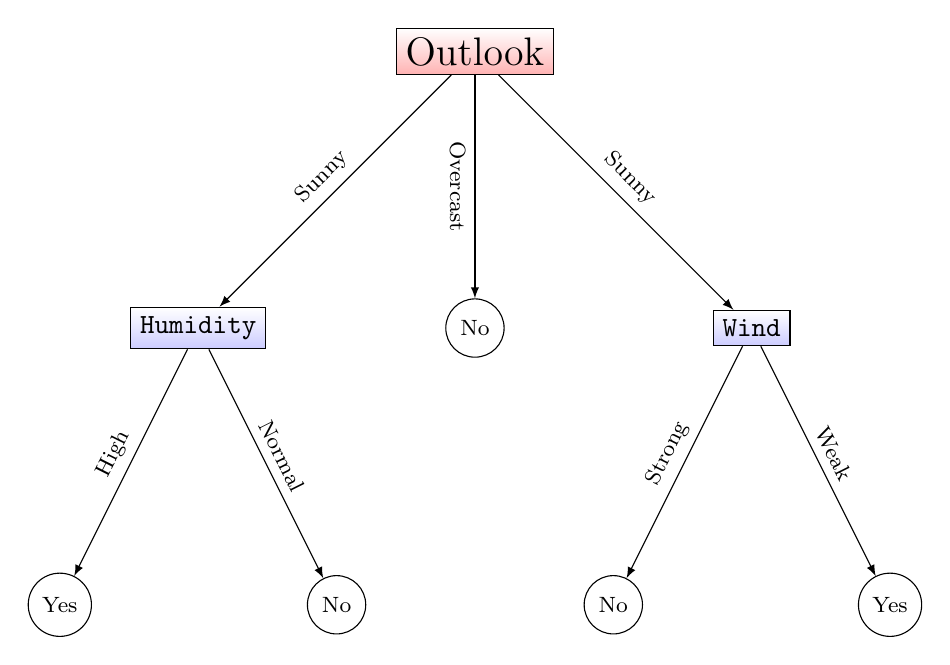
\begin{tikzpicture}
  [
    grow                    = down,
    sibling distance        = 10em,
    level distance          = 10em,
    edge from parent/.style = {draw, -latex},
    every node/.style       = {font=\footnotesize},
    sloped
  ]

\node [root] {Outlook}
    child { node [env] {Humidity}
       child { node [dummy] {Yes}
           edge from parent node [above] {High} }
       child { node [dummy] {No}
            edge from parent node [above] {Normal} }
    edge from parent node [above] {Sunny} }
    child { node [dummy] {No}
      edge from parent node [below] {Overcast} }
    child { node [env] {Wind}
       child { node [dummy] {No}
           edge from parent node [above] {Strong} }
       child { node [dummy] {Yes}
            edge from parent node [above] {Weak} }
    edge from parent node [above] {Sunny} };
\end{tikzpicture}
% \end{document}					
					\caption{Cây quyết định phân loại xem những buổi sáng thứ 7 nào sẽ có chơi Quần vợt (PlayTennis) (Tham khảo từ trang 53 của \cite{mltextbook})}
					\label{fig:tree}
				\end{figure}
				\par Cây quyết định (Decision Tree) là một mô hình học máy có giám sát, trong đó hàm mục tiêu được mô tả bằng một cây quyết định. Cây quyết định cũng có thể được biểu diễn lại dưới dạng một tập các luật giúp dễ đọc, dễ hiểu.
				\par Mỗi nút của cây biểu diễn một thuộc tính. Mỗi nhánh xuất phát từ nút đó thể hiện giá trị của thuộc tính đó. Một mẫu được phân loại trên cây quyết định bằng cách duyệt nó trên cây, bắt đầu từ gốc cho đến khi gặp giá trị phân loại (lá). 
				Cây quyết định ở Hình \ref{fig:tree} xét xem thử những buổi sáng thứ 7 nào sẽ có chơi quần vợt dựa trên các thuộc tính Outlook, Temperature, Humidity, Wind.
				\\Ví dụ mẫu (Outlook = Sunny, Temperature = Cold, Humidity = High, Wind = Strong) duyệt trên cây sẽ cho ra kết quả phân loại là mẫu âm (No). Cây quyết định này cũng có thể được biểu diễn lại thành luật, là hội của các tuyển:
				\begin{center}
					\begin{tabular}{l}				
						(Outlook = Sunny $\wedge$ Humidity = Normal)
						\\$\lor$ (Outlook = Overcast)
						\\$\lor$ (Outlook = Rain $\wedge$ Wind = Weak)
					\end{tabular}
				\end{center}											
			\subsection*{Giải thuật}		
				\par Phần lớn các giải thuật học trên cây quyết định (trong đó ID3 là giải thuật điển hình) đều theo hướng tiếp cận từ trên xuống, dùng giải thuật tham lam tìm kiếm trong không gian của tất cả các kết quả cây quyết định có thể xuất hiện. ID3 là giải thuật học cơ bản trên cây quyết định. Phần lớn các giải thuật học trên cây quyết định đều đi theo hướng tiếp cận của ID3, là sự mở rộng và nâng cấp của nó (trong đó có giải thuật C4.5).			
				\par Trong quá trình xây dựng cây từ trên xuống, ở mỗi bước cần xác định được thuộc tính nào là tốt nhất (được hiểu là thuộc tính phân loại hiệu quả nhất cho các mẫu) để làm gốc cho cây ở thời điểm đó. Sự lựa chọn thuộc tính tốt nhất được thực hiện nhờ vào độ đo \textit{Information Gain}.
				\begin{itemize}
					\item{Entropy: Là một hàm đo mức độ không thuần khiết (impurity) của tập mẫu, được sử dụng trong các giải thuật ID3, C4.5. Đối với các tập mẫu thuần khiết, giả sử tập mẫu gồm toàn mẫu âm hoặc dương (xét tập mẫu nhị phân), entropy sẽ bằng 0. Mặt khác đối với các tập mẫu "hỗn độn nhất", với số lượng mẫu âm và dương bằng nhau, entropy sẽ bằng 1. Giá trị của hàm entropy nói chung nằm trong đoạn [0,1] tùy theo số lượng mẫu của các loại. Ngoài ra, một số hàm đo khác (như Gini) có thể được sử dụng thay thể cho hàm Entropy.

					\begin{itemize}
						\item{Công thức Entropy:
						\\Xét tập S là tập mẫu nhị phân gồm các mẫu dương (+) và các mẫu âm (-). Khi đó:
						\begin{equation}					
						Entropy(S) \equiv -p_{(+)}log_{2}p_{(+)} - p_{(-)}log_{2}p_{(-)}
						\end{equation}}						
						\item{Ví dụ: Tập mẫu S gồm 14 mẫu nhị phân, trong đó có 8 mẫu dương và 6 mẫu âm.\\
						Tần số mẫu dương là: 8/14 \\
						Tần số mẫu dương là: 6/14 \\
					 	Khi đó entropy của tập S là:\\	
					 	\begin{align*}						
							Entropy(S) = -(8/14)log_{2}(8/14) - (6/14)log_{2}(6/14) = 0.985
						\end{align*}		
						}
					\end{itemize}}					
					\item{Information Gain: Là một hàm đo độ giảm entropy của tập mẫu khi phân đoạn nó trên một thuộc tính. Độ giảm entropy (độ giảm sự "không thuần khiết") càng cao thì phép phân đoạn đó càng hiệu quả.
					\begin{itemize}
						\item{Công thức Information Gain:
						\\Cho tập S và thuộc tính A. Khi đó: Information Gain của S trên A là:
						\begin{equation}
							\label{eq:gain}
							Gain(S,A) \equiv Entropy(S) - \sum_{v \in values(A)}\frac{|S_v|}{|S|}Entropy(S_v)
						\end{equation}}
						\item{Ví dụ: Tập mẫu S gồm 14 mẫu nhị phân, trong đó có 8 mẫu dương và 6 mẫu âm. 
						Thuộc tính A có 3 giá trị là A1, A2, A3. Thống kê cho thuộc tính A trên S như sau:
						\begin{table}[H]
							\centering							
							\label{my-label}
							\begin{tabular}{|l|l|l|l|}
							\hline
							             & A = A1 & A = A2 & A = A3 \\ \hline
							Số mẫu dương & 2      & 3      & 4      \\ \hline
							Số mẫu âm    & 2      & 2      & 1      \\ \hline
							\end{tabular}
							\caption{Ví dụ tính Information Gain}
						\end{table}
						$\begin{aligned}							
							Entropy(S) = -(8/14)log_{2}(8/14) - (6/14)log_{2}(6/14) = 0.985				
						\end{aligned}$	
						\\
						$\begin{aligned}							
							Entropy(S_{A_1}) = -(2/4)log_{2}(2/4) - (2/4)log_{2}(2/4) = 1				
						\end{aligned}$	
						\\
						$\begin{aligned}							
							Entropy(S_{A_2}) = -(3/5)log_{2}(3/5) - (2/5)log_{2}(2/5) = 0.970
						\end{aligned}$
						\\
						$\begin{aligned}							
							Entropy(S_{A_3}) = -(4/5)log_{2}(4/5) - (1/5)log_{2}(1/5) = 0.722
						\end{aligned}$	
						\\						
						\begin{align*}							
					    	Gain(S,A) &= Entropy(S) - ((4/14)*Entropy(S_{A_1}) + (5/14)*Entropy(S_{A_2}) \\
					    	&+ (5/14)*Entropy(S_{A_3})) = 0.095					    	
						\end{align*}														
						}						
					\end{itemize}}					
				\end{itemize}
				\begin{figure}[H]
					\centering
					% \documentclass{article}

% \begin{document}
% \begin{figure}
	\noindent\fbox{
	    \parbox{\textwidth}{
	        ID3\textit{(Examples, Targetattribute, Attributes)
			\\Examples are the training examples. Targetattribute is the attribute whose value is to be
			predicted by the tree. Attributes is a list of other attributes that may be tested by the learned
			decision tree. Returns a decision tree that correctly classiJies the given Examples.}
			\begin{itemize}
				\item{Create a \textit{Root} node for the tree}
				\item{If all \textit{Examples} are positive, Return the single-node tree \textit{Root}, with label = +}
				\item{If all \textit{Examples} are negative, Return the single-node tree \textit{Root}, with label = -}
				\item{If \textit{Attributes} is empty, Return the single-node tree \textit{Root}, with label = most common value of \textit{Targetattribute} in \textit{Examples}}
				\item{Otherwise Begin
					\begin{itemize}
						\item{A $\gets$ the attribute from \textit{Attributes} that best* classifies \textit{Examples}}
						\item{The decision attribute for \textit{Root} $\gets$ A}
						\item{For each possible value, $v_i$, of A,
							\begin{itemize}
							\item{Add a new tree branch below \textit{Root}, corresponding to the test A = $v_i$}
							\item{Let \textit{$Examples_{v_i}$} be the subset of Examples that have value $v_i$ for A}
							\item{If \textit{$Examples_{v_i}$} is empty
								\begin{itemize}
									\item{Then below this new branch add a leaf node with label = most common value of \textit{Targetattribute} in \textit{Examples}}
									\item{Else below this new branch add the subtree ID3(\textit{$Examples_{v_i}$ (Targetattribute, Attributes - \{A\}})}
								\end{itemize}}
							\end{itemize}}
					\end{itemize}}			
				\item{End}
				\item{Return Root}
			\end{itemize}
			}
		} 	
% \end{figure}
% \end{document}
					* The best attribute is the one with highest information gain, as defined in Equation 
					\ref{eq:gain}
					\caption{Giải thuật ID3 trong cây quyết định (Tham khảo từ trang 59 của \cite{mltextbook})}
					\label{fig:id3}
				\end{figure}
			\subsection*{Vấn đề Quá vừa dữ liệu}
				\par Giải thuật ở Hình \ref{fig:id3} là hợp lý trong một số trường hợp, nhưng thực tế nó có thể dẫn đến hiện tượng \textit{Quá vừa dữ liệu (Overfitting data)}. Điều này xảy ra là bởi vì giải thuật này chỉ cố gắng xây dựng cây đủ để phân loại đúng tập dữ liệu học, \textit{Quá vừa dữ liệu} sẽ xảy ra nếu dữ liệu trong tập dữ liệu học bị nhiễu hoặc chứa quá ít mẫu để có thể xấp xỉ đúng hàm mục tiêu.
				\par Một phương pháp phổ biến được sử dụng để giải quyết hiện tượng này là cho phép cây bị \textit{Quá vừa dữ liệu}, nhưng sau đó cắt tỉa (post-pruning). Trong phương pháp này, tập dữ liệu học được chia ra làm hai, một tập dữ liệu học (training set) và một tập kiểm chứng phép cắt tỉa (validation set). Cây sẽ được xây dựng dựa trên tập dữ liệu học trước, có 2 hướng giải quyết vấn đề cắt tỉa:
				\begin{itemize}
				\item{Cắt tỉa giảm lỗi (reduced error pruning): Cân nhắc từng nút của cây, và thực hiện cắt tỉa cây con có gốc là nút đó. Cây sau phép cắt tỉa này được đánh giá độ chính xác dựa vào tập kiểm thử, nếu độ chính xác không thấp hơn cây trước phép cắt tỉa thì cho phép cắt tỉa. Việc cắt tỉa được lặp lại với các nút không làm giảm độ chính xác của cây cho đến khi không còn lựa chọn nào.}
				\item{Cắt tỉa theo luật (rule post-pruning): Đây là phương pháp được sử dụng trong giải thuật C4.5, bao gồm các bước:
					\begin{itemize}
						\item{Xây dựng cây từ tập dữ liệu học}
						\item{Chuyển cây thành một tập các luật}
						\item{Cắt tỉa điều kiện (precondition) trong các luật sao cho độ chính xác không giảm (đối với C4.5, tính toán độ chính xác trên toàn bộ tập dữ liệu học)}
						\item{Sắp xếp tập các luật cuối cùng (sau khi cắt tỉa xong) theo độ chính xác và sử dụng các luật này để phân loại cho các mẫu mới (unseen data).}
					\end{itemize}}				
				\end{itemize}

	\chapter{Phương pháp đề xuất và hiện thực}	
		\section{Nội dung bài toán}
			\par Cho một văn bản chứa ý kiến gồm một tập các đối tượng O = \{$o_1$,$o_2$,$o_3$,...\}. Giả định của bài toán là ý kiến trong văn bản đều từ một chủ thể duy nhất và tập thuộc tính $F_i$ của các đối tượng đã được tìm ra. Mục tiêu của bài toán là tìm các chuỗi đồng tham chiếu đồng nhất (identity) của đối tượng và thuộc tính.
			\begin{itemize}
				\item{Đầu vào: Văn bản có chứa ý kiến.}
				\item{Giả định:
				\begin{itemize}
					\item{Ý kiến trong văn bản đến từ một chủ thể duy nhất.}
					\item{Các \textit{synonyms} của thuộc tính (bao gồm bản thân đối tượng) đã được tìm ra.}
					\item{Quan hệ đồng tham chiếu thuộc dạng đồng nhất (identity).}
				\end{itemize}}
				\item{Đầu ra: Các chuỗi đồng tham chiếu của đối tượng và thuộc tính.}
			\end{itemize}
			\par Ví dụ: Cho văn bản \\
			\par \textit{I don't like where the power button(1) of Lumia 920(2) is. The battery life(3) is rather poor. I charge it(4) every night and still have had it(5) die on my twice in less than a month. Lumia 920(6) takes great pictures(7). The screen(8) is very sharp and it(9) is easy to watch videos(10) on. However, I want to admit the Lumia(11) is by far better than the iPhone(12)! Learn how to use, and it(13)'s amazing!}	
			\begin{itemize}		
			\item{Tập các đối tượng trong văn bản trên (Các cụm danh từ riêng): \{Lumia 920 (2), Lumia 920(6), the Lumia(11), iPhone(12)\}}
			\item{Giả định đã tìm được tập các synonyms thuộc tính trong văn bản trên: \{the power button(1), the battery life(3), pictures(7), the screen(8), videos(10)\}}
			\item{Đầu ra của bài toán là các chuỗi đồng tham chiếu cho đối tượng và thuộc tính:						
				\begin{center}
					\begin{tabular}{l}
						\{the power button(1)\}
						\\\{Lumia 920(2), it(4), it(5), Lumia 920(6), it(13), the Lumia(11)\}
						\\\{the battery life(3)\}
						\\\{pictures(7)\}
						\\\{the screen(8), it(9)\}
						\\\{videos(10)\}
						\\\{iPhone(12)\}
					\end{tabular}
			 	\end{center}}
		 	\end{itemize}
		\section{Tổng quan quy trình}
			\begin{figure}[H] 
				\centering				
				\resizebox{160mm}{!}{% Author: Rasmus Pank Roulund
% \documentclass{minimal}
% \usepackage{tikz}
% \usepackage[utf8]{vietnam}

% \begin{document}
% \usetikzlibrary{arrows,chains,positioning,scopes}

\tikzset{
    block/.style={draw,thick,text width=10em,minimum height=6.5em,minimum width=11em,align=center},
    arrow/.style={->, thick}
}
\begin{tikzpicture}
  {[start chain]
      \node[block,on chain] (N1) {Tập hợp các cụm danh từ};
      \node[block,on chain,join=by {arrow},right=1cm of N1] (N2) {Tiền xử lý};
      \node[block,on chain,join=by {arrow},right=1cm of N2] (N3) {Trích xuất cụm danh từ};
      \node[block,on chain,join=by {arrow},below=1cm of N3] (N4) {Xây dựng dữ liệu học và kiểm tra};
      \node[block,on chain,join=by {arrow},left=1cm of N4] (N5) {Xây dựng bộ phân loại và gom cụm};
      \node[block,on chain,join=by {arrow},left=1cm of N5] (N6) {Các chuỗi đồng tham chiếu};      
    }
      
  \end{tikzpicture}
% \end{document}}
				\caption{Tổng quan quy trình phân giải đồng tham chiếu}							
			\end{figure}			
		\section{Tiền xử lý}
		\subsection*{Tiền xử lý văn bản thô}
		\par Dữ liệu thu thập được sẽ được tiền xử lý nhằm giúp giảm sai số cho các bước sau. Bước tiền xử lý đảm bảo đặc tính ngôn ngữ của văn bản không thay đổi. Sau đây trình bày một số thao tác tiền xử lý mà chúng tôi đã thực hiện:
		\begin{itemize}
			\item{Tiền xử lý các lỗi liên quan đến đặc tính của công cụ Stanford
				\par Ví dụ: "I am very pleased with the phone we received.It is a genuine Samsung S3". Từ đầu tiên của câu sau phải cách dấu chấm của câu trước ít nhất một khoảng trắng, trong trường hợp như trên, nếu "It" trong câu 2 nằm ngay sau dấu "." của câu trước nó, công cụ sẽ bắt cả 2 thành chỉ 1 câu, làm cho quá trình phân tích cú pháp (parse) ngay sau đó bị sai.}
			\item{Tiền xử lý các lỗi liên quan đến ngữ pháp của văn bản: Một số câu trong dữ liệu thu thập có thể "sai" ngữ pháp (có thể là do văn phạm của người viết review không thực sự chuẩn xác). 
				\par Ví dụ: "Yes it was hard to see the screen in daylight but I don't expect to see a crystal clear picture on a cell phone, they aren't mini laptops folks". ("Yes" được dùng ở đầu câu không hợp lý, công cụ bắt "Yes it" là cụm danh từ).			
				\par "I had low expectations about this phone, but when I opened it for the first time I knew it was tend to be mine". ("was tend" sai ngữ pháp)
				\par Những cú pháp văn phạm sai như vậy làm cho công cụ parsing sai. Hiện tại, với việc thực hiện trên một khối lượng dữ liệu khá nhỏ, trong lúc chọn lọc review chúng tôi cố gắng đọc và tìm ra các review có cấu trúc văn phạm tiếng Anh đúng, hoặc cố gắng sửa các lỗi nhỏ trong câu để câu được hoàn thiện ngữ pháp. Tuy nhiên, nếu áp dụng trên một khối lượng dữ liệu lớn hơn, những lối văn phạm này sẽ gây ảnh hưởng.} 
		\end{itemize}

		\subsection*{Tách câu, tách từ và gán nhãn từ loại}
			\par Việc tách câu, tách từ đóng vai trò quan trọng trong các bước tiếp theo. Những công việc này thực hiện được là nhờ vào gói công cụ Stanford \footnote{http://stanfordnlp.github.io/CoreNLP}. Các nhãn từ loại (part-of-speech) cũng được trích ra nhờ vào gói công cụ này, chúng được sử dụng theo như Penn Treebank POS Tag \footnote{http://web.mit.edu/6.863/www/PennTreebankTags.html}.

		\section{Trích xuất cụm danh từ}
			\subsection*{Tìm và lọc các cụm danh từ}
				\par Như đã đề cập ở mục \ref{coref_problem}, các \textit{mention} trong bài toán đồng tham chiếu thường là các danh từ/cụm danh từ (từ đây gọi chung là cụm danh từ). Mặt khác trong các văn bản chứa ý kiến, các đối tượng và thuộc tính hầu hết cũng đều được thể hiện bằng các cụm danh từ. Do đó, để trích xuất ra các \textit{mention} phục vụ cho các bước tiếp theo, chúng tôi thực hiện trích xuất các cụm danh từ trong văn bản. Để thực hiện việc này, trước tiên dùng công cụ Stanford để gán nhãn từ loại cho văn bản rồi sau đó tìm các cụm danh từ dựa vào công cụ CRFChunker \cite{crfchunker}. Tập hợp các cụm danh từ được tìm ra gồm ba loại: các cụm danh từ chỉ đối tượng (cụm danh từ riêng), các cụm danh từ chỉ thuộc tính, các cụm danh từ khác.
				\par Trong nhóm các cụm danh từ khác đã được tìm ra, có những cụm danh từ sẽ không được đưa vào bộ phân loại vì chúng không thể chỉ về đối tượng và thuộc tính. Đó là những cụm danh từ thuộc các loại sau:
					\begin{itemize}
						\item{Các cụm danh từ chỉ dùng nói để nói đến con người: Là các cụm danh từ mà HEAD của chúng thuộc về danh sách sau:
						\par \textit{i;me;myself;we;us;ourselves;you;yourself;yourselves;he;him;himself;
						\\she;her;herself;anyone;someone;somebody;everyone;anybody;everybody;nobody;people}}
						\item{Các cụm danh từ dùng để nói về thời gian: Là các cụm danh từ mà HEAD của chúng thuộc về danh sách sau:
						\par \textit{minute;minutes;hour;hours;day;days;week;weeks;month;months;year;years;
						\\january;february;march;april;may;june;july;august;september;october;november;
						\\december;monday;tuesday;wednesday;thursday;friday;saturday;sunday}}
						\item{Các cụm danh từ dùng để nói về số lượng: Là các cụm danh từ mà HEAD của chúng thuộc về danh sách sau:
						\par \textit{lot;lots;number;total;amount;little;much;many;ton;tons;plenty;some;bit;a}}
						\item{Các cụm danh từ chỉ mốc thời gian: 2PM, 4PM, 5 o'clock.}
						\item{Một số cụm danh từ khác: \textit{there}, \textit{oh}, \textit{etc}, ...}					
					\end{itemize}
				\par Nói về khái niệm HEAD. HEAD của một cụm từ là từ chính của cụm từ đó, nó quyết định dạng cú pháp của cụm từ. Đối với cụm danh từ, HEAD thường là danh từ hoặc đại từ. Ví dụ: Cụm danh từ \textit{the next October} có HEAD là từ \textit{October}.
				\par Sau đây trình bày một ví dụ về bước trích xuất cụm danh từ:
					\\\textit{The Note 3 is a lot lighter than my HTC EVO. It's very fast and has so many features that an IPhone5 can't touch. I love the camera features and it takes great pictures.}
					\\Dùng công cụ Stanford để gán nhãn từ loại và dùng CRFChunker để ghép cụm cho đoạn văn bản trên, ta có kết quả như sau:

					\begin{figure}[H]
						\centering				
						\noindent\fbox{
						    \parbox{\textwidth}{
						        It/PRP/B-NP 's/VBZ/B-VP very/RB/B-ADJP fast/JJ/I-ADJP and/CC/O has/VBZ/B-VP so/RB/B-NP many/JJ/I-NP features/NNS/I-NP that/IN/B-SBAR an/DT/B-NP IPhone5/NN/I-NP ca/MD/B-VP n't/RB/I-VP touch/VB/I-VP ././O 
						        \\
						        \\
								I/PRP/B-NP love/VBP/B-VP the/DT/B-NP camera/NN/I-NP features/NNS/I-NP and/CC/O it/PRP/B-NP takes/VBZ/B-VP great/JJ/B-NP pictures/NNS/I-NP ././O
					    	}
						}
						\caption{Kết quả đầu ra của công cụ CRFChunker}
					\end{figure}

					\par Đọc và lưu thông tin từ đoạn kết quả ghép cụm này, sau đó bỏ đi các cụm danh từ như đã nói ở trên, có được các cụm danh từ sẽ được dùng cho các bước tiếp theo:\\
					\textit{<The Note 3> is a lot lighter than <my HTC EVO>. <It>'s very fast and has <so many features> that <an IPhone5> can't touch. I love <the camera features> and <it> takes <great pictures>.}
					\\Các cụm từ trong dấu <> là các cụm danh từ được trích xuất và sử dụng cho các bước tiếp theo.

			\subsection*{Gán nhãn cho cụm danh từ}
				\par Kết quả của bước trích xuất cụm danh từ là cơ sở cho việc gán nhãn dữ liệu. Mục đích của việc gán nhãn dữ liệu là xác định loại của các cụm danh từ đã được tìm ra, liệu chúng có chỉ đến đối tượng, thuộc tính không và đồng thời nếu có thì biểu diễn sự đồng tham chiếu đó. Do vậy việc tạo tập dữ liệu để hệ thống học và kiểm tra sẽ dễ dàng hơn.
				\par Mỗi cụm danh từ được gán nhãn có dạng <ID,REF,TYPE NP>. Trong đó:
					\begin{itemize}
						\item{ID: là giá trị nguyên dương duy nhất được gán cho mỗi cụm danh từ, dùng để chỉ vị trí của cụm danh từ trong câu.}
						\item{REF: là giá trị ID của cụm danh từ mà cụm danh từ hiện tại đang  tham chiếu đến.}
						\item{TYPE: là giá trị dùng để phân loại cụm danh từ. 
							\begin{itemize}
								\item{TYPE = 0 nếu cụm danh từ là tên đối tượng}
								\item{TYPE = 3 nếu cụm danh từ là thuộc tính}
								\item{TYPE = 1 nếu cụm danh từ không phải chỉ thuộc tính hoặc đối tượng. Cụm danh từ nào có TYPE là 1 thì giá trị REF của nó là 0.}
								\item{TYPE = 2 nếu cụm danh từ dùng để đại diện cho đối tượng, thuộc tính.}
							\end{itemize}}
						\item{ID: là giá trị nguyên dương duy nhất được gán cho mỗi cụm danh từ, dùng để chỉ vị trí của cụm danh từ trong câu.}
						\item{NP: cụm danh từ.}
					\end{itemize}
				\par Ví dụ: Đoạn văn sau đã được gán nhãn
					\\<0,-1,0 The Note 3> is a lot lighter than <1,-1,0 my HTC EVO>. <2,0,2 It>'s very fast and has <3,0,1 so many features> that <4,-1,0 an IPhone5> can't touch. I love <5,-1,3 the camera > and <6,5,2 it> takes <7,-1,3 great pictures>.
					\\Giải thích: 
					\begin{itemize}
						\item{Các cụm danh từ <0,-1,0 The Note 3>, <1,-1,0 my HTC EVO> và <4,-1,0 an IPhone5> là tên đối tượng (TYPE = 0).}
						\item{<3,0,1 so many features> là cụm danh từ mà không chỉ đối tượng hay thuộc tính (TYPE = 1).}
						\item{<2,0,2 It> và <6,5,2 it> là cụm danh từ đại diện cho đối tượng thuộc tính (TYPE = 2). Trong đó: <2,0,2 It> chỉ đối tượng <0,-1,0 The Note 3> vì có REF = 0; <6,5,2 it> chỉ thuộc tính <5,-1,3 the camera> vì có REF = 5.}
						\item{<5,-1,3 the camera > và <7,-1,3 great pictures> là tên thuộc tính (TYPE = 3).}
					\end{itemize} 
				
				\begin{figure}[H]
					\centering							
					\indent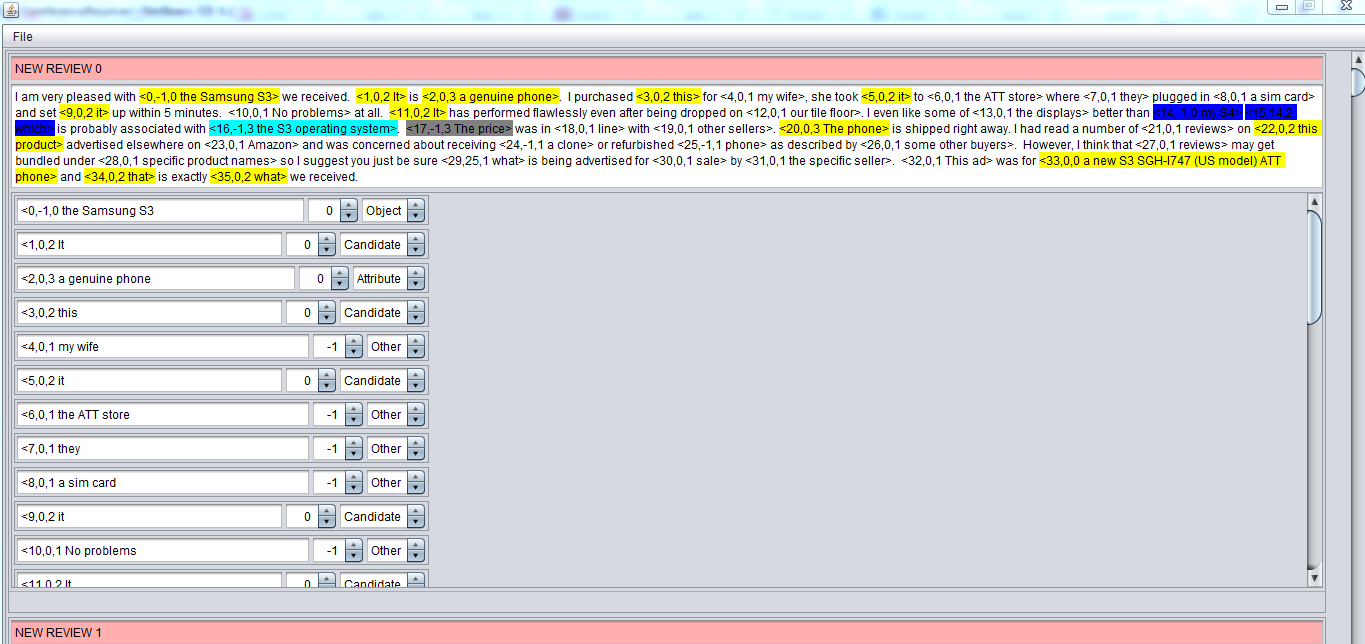
\includegraphics[scale=0.45]{images/markup_tool}				
					\caption{Công cụ gán nhãn dữ liệu đồng tham chiếu}	
				\end{figure}				

				\par Gán nhãn bằng tay là công việc chứa đựng nhiều nguy cơ sai sót, đặc biệt trên một khối lượng dữ liệu lớn. Do vậy, nhằm tránh những lỗi sai và đồng thời tăng tốc độ làm việc, chúng tôi đã viết một công cụ giúp gán nhãn dữ liệu bằng Java kết hợp với gói giao diện Swing. Công cụ này lấy đầu vào là các văn bản đã được trích xuất cụm danh từ và xuất ra văn bản được gán nhãn như ví dụ này. Bằng các thao tác kích chuột đơn giản, có thể chọn TYPE và chuỗi đồng tham chiếu (các cụm danh từ chung chuỗi thì chung màu) cho các cụm danh từ, sau đó xuất kết quả (Export).
		
		\section{Tạo tập dữ liệu học và kiểm tra}
			\subsection*{Tạo tập dữ liệu học}
				\par Giải thuật phân loại nhận đầu vào để học là một tập các mẫu. Một mẫu dùng để học (instance) có dạng: Instance = (<$f_1$,$f_2$,…,$f_n$>, $y$), trong đó $n$ thể hiện mẫu có $n$ thuộc tính, $f_i$ thể hiện giá trị của thuộc tính thứ $i$, $y$ thể hiện giá trị phân loại đầu ra của mẫu. Cứ mỗi cặp (NP1, NP2) tạo được một mẫu. 
				\\Từ tập dữ liệu học, ta xác định được danh sách L chứa các cụm danh từ NPs.
				\par Tập mẫu dùng để học (Instances): mọi cặp (NP1, NP2) được tạo ra từ danh sách L và thỏa mãn điều kiện NP1 hoặc NP2 là cụm danh từ là tên đối tượng/thuộc tính (TYPE = 0 hoặc TYPE = 3). Lí do vì đề tài chỉ thực hiện với mục đích phân giải đồng tham chiếu cho các đối tượng/thuộc tính đã biết.
				\\Đặc điểm mỗi mẫu dữ liệu để học:
				\begin{itemize}
					\item{Tập thuộc tính: đã được đề cập ở bảng 5.1.}
					\item{Giá trị phân loại: (NP1, NP2) được gán nhãn phân loại là true nếu:
						\begin{itemize}
							\item{TYPE của NP1 và NP2 là 0 hoặc 2 hoặc 3 (NP1 và NP2 là cụm danh từ chỉ đối tượng hoặc thuộc tính).}
							\item{Giá trị REF của NP2 bằng giá trị REF của NP1 hoặc giá trị REF của NP2 bằng giá trị ID của NP1. (NP1, NP2) nhận giá trị false trong những trường hợp còn lại.}
						\end{itemize}}
				\end{itemize}
				\par Hình 5.4 trình bày một tập gồm các mẫu dữ liệu học được tạo ra từ một đoạn văn.		
				\begin{figure}[H]
					\centering	
					\large			
					\noindent\fbox{
					    \parbox{\textwidth}{
					    \sffamily{
					        0,4,6,false,false,true,false,1,true,false,false,false,2,false,false,false,false,10,false,false
							0,0,6,false,false,true,false,3,true,false,false,false,2,false,false,false,false,10,false,false
							0,4,5,false,false,true,false,1,true,false,false,false,2,false,false,false,false,10,false,false
							0,0,5,false,false,true,false,3,true,false,false,false,2,false,false,false,false,10,false,true
							0,3,4,true,false,false,false,0,true,false,true,false,2,false,false,false,false,1,false,false
							0,2,4,true,false,false,false,1,true,false,false,false,2,false,false,false,false,1,false,false
							0,1,4,false,false,false,false,2,true,false,false,false,2,false,false,false,false,4,false,false
							0,0,4,false,false,false,false,2,true,false,false,false,2,false,false,false,false,0,false,false
							0,0,3,false,true,false,false,2,true,false,false,false,2,false,false,false,false,10,false,true
							0,0,2,false,true,false,false,1,true,false,false,false,2,false,false,false,false,10,false,true
							0,0,1,false,false,false,false,0,true,false,false,false,2,true,false,false,false,10,false,false}
				    	}
					}
					\caption{Các mẫu dữ liệu học được tạo ra bởi đoạn văn: \textit{I have owned <0,-1,0 the Nokia 6101> since <1,0,1 late October 2005>. I absolutely love <2,0,2 it>! <3,0,2 It> has <4,-1,3 a good camera>. I wouldn't trade <5,0,2 the phone> for <6,0,1 the world>.
}. Mỗi hàng chính là một mẫu. Ý nghĩa của các giá trị từ trái sang phải trong mỗi mẫu là: ID\_NP1, ID\_NP2, NP1\_PRONOUN, NP2\_PRONOUN, DEF\_NP2, DEM\_NP2, DISTANCE, NUMBER\_AGREEMENT, IS\_BETWEEN, HAS\_BETWEEN, SENTIMENT\_CONSISTENCY, PROPER\_NAME, SUBSTRING, HEAD\_MATCH, EXACT\_MATCH, OPINION\_WORD, RELATIVE\_PRONOUN, COREF. Trong đó, COREF là giá trị phân loại của mẫu trên thực tế.}
				\end{figure}
				\subsection*{Tạo tập dữ liệu học}
				\par Cách tạo tập dữ liệu kiểm tra hoàn toàn giống với cách tạo tập dữ liệu học.

			\subsection*{Tạo các vectơ đặc trưng}

				\begin{table}[H]
					\centering
					\begin{tabular}{|l|l|l|}
\hline
Nhóm thuộc tính                                                                               & Thuộc tính                                                                           & Giải thích                                                                                                                                                                                                                                   \\ \hline
\multirow{2}{*}{\begin{tabular}[c]{@{}l@{}}Nhóm liên quan \\ khai khoáng ý kiến\end{tabular}} & Tính nhất quán về ý kiến                                                             & \begin{tabular}[c]{@{}l@{}}Bằng 1 nếu NP1 và NP2 có\\ cùng thiên hướng ý kiến. \\ Bằng 0 nếu chúng khác về \\ thiên hướng ý kiến. \\ Nếu không xác định được \\ thiên hướngý kiến cho NP1 \\ hoặc NP2 thì bằng 2.\end{tabular} \\ \cline{2-3} 
                                                                                              & \begin{tabular}[c]{@{}l@{}}Sự kết hợp giữa thực thể \\ và từ chỉ ý kiến\end{tabular} & \begin{tabular}[c]{@{}l@{}}Bằng 0,1,2,3,4,10 tùy vào \\ xếp hạng PMI\end{tabular}                                                                                                                                                            \\ \hline
\multirow{6}{*}{\begin{tabular}[c]{@{}l@{}}Nhóm liên quan \\ ngữ pháp\end{tabular}}           & NP1 là đại từ                                                                    & \begin{tabular}[c]{@{}l@{}}Bằng 1 nếu NP1 là đại từ, \\ ngược lại bằng 0\end{tabular}                                                                                                                                                    \\ \cline{2-3} 
                                                                                              & NP2 là đại từ                                                                     & \begin{tabular}[c]{@{}l@{}}Bằng 1 nếu NP2 là đại từ, \\ ngược lại bằng 0\end{tabular}                                                                                                                                                     \\ \cline{2-3} 
                                                                                              & Tính thống nhất về số                                                                & \begin{tabular}[c]{@{}l@{}}Bằng 1 nếu NP1 và NP2 \\ thống nhất về số (trong ngữ pháp),\\  ngược lại bằng 0\end{tabular}                                                                                                               \\ \cline{2-3} 
                                                                                              & Từ hạn định                                                                          & \begin{tabular}[c]{@{}l@{}}Bằng 1 nếu NP2 bắt đầu bằng \\ "the", ngược lại bằng 0\end{tabular}                                                                                                                                            \\ \cline{2-3} 
                                                                                              & Từ chỉ trỏ                                                                           & \begin{tabular}[c]{@{}l@{}}Bằng 1 nếu NP2 bắt đầu bằng \\ "this", "that", "these", those", \\ ngược lại bằng 0\end{tabular}                                                                                                               \\ \cline{2-3} 
                                                                                              & \begin{tabular}[c]{@{}l@{}}Cả NP1 và NP2 \\ đều là tên riêng\end{tabular} & \begin{tabular}[c]{@{}l@{}}Bằng 1 nếu NP1 và NP2 \\ đều là tên riêng, ngược lại \\ bằng 0\end{tabular}                                                                                                                            \\ \hline
\begin{tabular}[c]{@{}l@{}}Nhóm liên quan \\ từ vựng\end{tabular}                             & Tương tự về từ vựng                                                                  & \begin{tabular}[c]{@{}l@{}}Tính tương tự về mặt từ vựng \\ (trùng hoặc gần giống nhau)\end{tabular}                                                                                                                                          \\ \hline
\multirow{3}{*}{Khác}                                                                         & Khoảng cách                                                                          & \begin{tabular}[c]{@{}l@{}}Khoảng cách về câu chứa NP1 \\ và NP2. Nếu chúng nằm cùng \\ một câu thì bằng 0\end{tabular}                                                                                                               \\ \cline{2-3} 
                                                                                              & Từ khóa "is" nằm ở giữa                                                              & \begin{tabular}[c]{@{}l@{}}Bằng 1 nếu có "is" không đi kèm \\ với chỉ định so sánh nào nằm ở \\ giữa NP1 và NP2, ngược lại \\ thì bằng 0\end{tabular}                                                                                 \\ \cline{2-3} 
                                                                                              & Từ khóa "has" nằm ở giữa                                                             & \begin{tabular}[c]{@{}l@{}}Bằng 1 nếu có "has" nằm ở giữa \\ NP1 và NP2, ngược lại thì \\ bằng 0\end{tabular}                                                                                                                         \\ \hline
\end{tabular}
					\caption{Các đặc trưng được sử dụng trong hệ thống}
					\label{features_table}
				\end{table}

				\par Giả sử các cặp \textit{mention} gồm hai cụm danh từ (NP1, NP2). Sau đây trình bày về các đặc trưng được sử dụng trong hệ thống.

				\subsubsection*{Đặc trưng Khoảng cách (DISTANCE)}
					\par \textit{Giải thích:} Là khoảng cách giữa hai cụm danh từ.
					\par \textit{Giá trị:} [0,1,2,3,…]. Nếu hai cụm danh từ nằm trong cùng một câu thì DISTANCE = 0; nếu hai cụm danh từ nằm trong hai câu liền nhau thì DISTANCE = 1; nếu giữa hai cụm danh từ có n câu (không tính hai câu chứa hai cụm danh từ đó và n > 0) thì DISTANCE = n + 1;
	 
				\subsubsection*{Đặc trưng NP1 là đại từ (NP1\_PRONOUN)}
					\par \textit{Giải thích:} Là khả năng cụm danh từ NP1 là đại từ.
					\par \textit{Giá trị:} [true, false] Thuộc tính nhận giá trị true nếu NP1 là đại từ và ngược lại nhận giá trị false. Đại từ được nhắc đến bao gồm: đại từ phản thân (itself, themselves), tân ngữ (it, them), đại từ nhân xưng (it, they) và tính từ sở hữu (its, their).

				\subsubsection*{Đặc trưng NP2 là đại từ (NP2\_PRONOUN)}
					\par \textit{Giải thích:} Là khả năng cụm danh từ NP2 là đại từ.
					\par \textit{Giá trị:} [true, false]. Thuộc tính nhận giá trị true nếu NP2 là đại từ và ngược lại nhận giá trị false.

				\subsubsection*{Đặc trưng Giống nhau hoàn toàn (EXACT\_MATCH)}
					\par \textit{Giải thích:} Là sự giống nhau hoàn toàn giữa hai cụm danh từ.
					\par \textit{Giá trị:} [true, false]. Thuộc tính nhận giá trị true nếu hai cụm danh từ giống nhau hoàn toàn và nhận giá trị false nếu ngược lại.

				\subsubsection*{Đặc trưng Danh từ chính giống nhau (HEAD\_MATCH)}
					\par \textit{Giải thích:} Là sự giống nhau giữa hai cụm danh từ.
					\par \textit{Giá trị:} [true, false]. Thuộc tính nhận giá trị true nếu danh từ chính của hai cụm danh từ giống nhau và nhận giá trị false nếu ngược lại.

				\subsubsection*{Đặc trưng Chuỗi con của nhau (SUBSTRING)}
					\par \textit{Giải thích:} Kiểm tra hai cụm danh từ có phải là chuỗi con của nhau hay không.
					\par \textit{Giá trị:} [true, false]. Thuộc tính nhận giá trị true nếu hai cụm danh từ là chuỗi con của nhau và nhận giá trị false nếu ngược lại.

				\subsubsection*{Đặc trưng Từ hạn định (DEF\_NP2)}
					\par \textit{Giải thích:} Là khả năng cụm danh từ NP2 là cụm danh từ xác định (cụm danh từ có từ bắt đầu là "the"). 
					\par \textit{Giá trị:} [true, false]. Thuộc tính nhận giá trị true nếu NP2 là cụm danh từ xác định và false nếu ngược lại.

				\subsubsection*{Đặc trưng Từ chỉ trỏ (DEM\_NP2)}
					\par \textit{Giải thích:} Là khả năng cụm danh từ NP2 là cụm danh từ xác định (cụm danh từ có từ bắt đầu là "this", "that", "these" hoặc "those"). 
					\par \textit{Giá trị:} [true, false]. Thuộc tính nhận giá trị true nếu NP2 là cụm danh từ chỉ định và false nếu ngược lại.

				\subsubsection*{Đặc trưng Tên riêng (PROPER\_NAME)}
					\par \textit{Giải thích:} Là khả năng cả hai cụm danh từ đều là tên riêng.
					\par \textit{Giá trị:} [true, false]. Thuộc tính nhận giá trị true nếu cả hai cụm danh từ đều là tên riêng và nếu không phải thì nhận giá trị false.
					\par \textit{Phương pháp hiện thực:} Phần sau trình bày cách mà chúng tôi đã sử dụng để xác định một cụm danh từ có là tên riêng hay không.				
					\par Một cụm danh từ gồm nhiều từ, thông qua công cụ gán nhãn từ loại (part of speech) của Stanford, biết được nhãn POS được gán với mỗi từ. Theo như quy ước về nhãn từ loại: Nhãn NNP chỉ danh từ riêng số ít, nhãn NNPS chỉ danh từ riêng số nhiều. Nếu nhãn của một từ nào đó trong cụm danh từ là NNP hoặc NNPS thì cụm danh từ đó là danh từ riêng. Ví dụ: Trong câu \textit{"The Galaxy S3 is beautiful."}, cụm danh từ The Galaxy S3 được công cụ gán nhãn của Stanford xử lý thành The/DT Galaxy/NNP S3/NNP. The Galaxy S3 là tên riêng vì có có từ Galaxy và từ S3 được gán nhãn NNP.
					\par Tuy nhiên, trên thực tế vẫn có nhiều danh từ riêng không tuân theo quy luật trên, dựa vào công cụ của Stanford không xác định được. Ví dụ: "iphone 6", "iPhone 6" hay "The 620", "the Active". Những cụm danh từ này công cụ gán nhãn từ loại của Stanford không gán được nhãn NNP hay NNPS. Vì vậy chúng tôi đề xuất hướng giải quyết:
					\begin{itemize}
						\item{Cụm danh từ có danh từ chính với nhãn là NNP, NNPS, CD được xác định là danh từ riêng. Như vậy với trường hợp "The 620", hệ thống vẫn sẽ nhận ra được là danh từ riêng vì có danh từ chính "620" mang nhãn CD.}
						\item{Tạo danh sách chứa các cụm danh từ riêng đặc biệt là \{"iphone", "iphones", "ipod", "ipad", "ipads"\}, nếu cụm danh từ có danh từ chính là một trong những từ nằm trong danh sách trên thì cụm danh từ đó là danh từ riêng.}
						\item{Nếu danh từ chính của cụm danh từ không được viết hoa thì cụm danh từ đó không phải là danh từ riêng.}
						\item{Nếu cụm danh từ có cụm danh từ chính viết hoa và danh từ chính đó không nằm trong từ điển thì được xác định là cụm danh từ riêng.}
						\item{Nếu cụm danh từ có danh từ chính viết hoa và danh từ chính nằm trong từ điển thì xét 2 trường hợp. Nếu cụm danh tử gồm hơn 1 từ thì cụm danh từ đó là danh từ riêng. Ví dụ: "The Active" là danh từ riêng. Nếu cụm danh từ chỉ là 1 từ thì không phải là danh từ riêng. Ví dụ: "It", "They" không phải là danh từ riêng.}
					\end{itemize}

				\subsubsection*{Đặc trưng Từ chỉ ý kiến (OPINION\_WORD)}
					\par \textit{Giải thích:} Là quan hệ giữa từ chỉ ý kiến của cụm danh từ NP1 với cụm danh từ NP2.
					\par \textit{Giá trị:} [0,1,2,3,4,10]. 
					\par Từ chỉ ý kiến là danh từ, tính từ hoặc trạng từ thường được dùng để đánh giá một thuộc tính, đối tượng (như đã đề cập trong mục \ref{ow_section}). Ví dụ: với câu "This phone is awesome", từ chỉ ý kiến là "awesome".
					\par Xuất phát từ ý tưởng: những từ chỉ ý kiến thường đi kèm với một số đối tượng, thuộc tính nhất định. Nếu từ chỉ ý kiến đi kèm với cụm danh từ NP1 và nó không bao giờ đi kèm với cụm danh từ NP2 thì dễ dàng thấy rằng khả năng NP1 và NP2 đồng tham chiếu với nhau là rất thấp. Ví dụ đoạn review sau: "The phone does not hold a charge long enough to last the day and it’s expensive." Ta thấy "long" thường được đi kèm với cụm danh từ "a charge" và ít khi đi kèm với cụm danh từ "the phone", nên "a charge" không đồng tham chiếu đến "the phone".
					\par \textit{Giải thuật:}
					\\Để xác định mối quan hệ giữa một từ chỉ ý kiến (OW) với một cụm danh từ (NP), chúng tôi sử dụng giá trị thông tin chung dựa trên điểm (pointwise mutual information PMI) được tính dựa vào OW và NP. Để xác định mối quan hệ giữa OW và NP, cần một tập dữ liệu T gồm các bài đánh giá chứa OW và NP đó. Khi đã có OW, NP và tập dữ liệu T, chúng tôi sẽ lần lượt tính các giá trị xác suất P(NP), P(OW), P(NP,OW). Trong đó:
					\begin{itemize} 
						\item{P(NP): Xác suất cụm danh từ xuất hiện trong tập dữ liệu T.}
						\item{P(OW): Xác suất từ chỉ ý kiến xuất hiện trong tập dữ liệu T.}
						\item{P(NP,OW): Xác suất cụm danh từ và từ chỉ ý kiến cùng xuất hiện trong một câu trong tập dữ liệu T.}
					\end{itemize}
					\par Công thức tính các giá trị P(OW), P(NP), O(NP,OW):
					\begin{itemize}
						\item{Công thức tính P(NP):
							\begin{equation*}
							P(NP) = \frac{NumOfS(NP)}{TotalSentences}
							\end{equation*}
						\\Trong đó \textit{NumOfS(P)} là số câu trong T chứa cụm danh từ NP và \textit{TotalSentences} là tổng số câu trong tập dữ liệu T.}
						\item{Công thức tính P(OW):
							\begin{equation*}
							P(OW) = \frac{NumOfS(OW)}{TotalSentences}
							\end{equation*}
						\\Trong đó \textit{NumOfS(OW)} là số câu trong T chứa cụm danh từ OW.}
						\item{Công thức tính P(NP,OW):
							\begin{equation*}
							P(NP,OW) = \frac{NumOfS(NP,OW)}{TotalSentences}
							\end{equation*}
						\\Trong đó \textit{NumOfS(NP,OW)} là số câu trong tập dữ liệu T chứa đồng thời NP và OW.}
					\end{itemize}
					\par Khi đã có các giá trị P(NP), P(OW), P(NP,OW) cần thiết, ta tính giá trị mối quan hệ giữa OW với NP theo công thức:
					\begin{center}
						\begin{equation*}
						PMI(NP,OW) = log\frac{(P(NP,OW)}{P(NP)\times P(OW)}
						\end{equation*}
					\end{center}
					\par Giá trị PMI không chỉ biểu hiện mối quan hệ giữa một OW và một NP, mà còn cho ta thấy mối quan hệ giữa cụm danh từ mà OW đang nói đến với NP. Do đó, từ giá trị PMI tính được, chúng tôi tạo thuộc tính mới OPINION\_WORD cho mỗi mẫu để biểu thị mối quan hệ giữa cặp hai cụm danh từ. Dưới đây là cách hiện thực của chúng tôi: 
					\par Cụm danh từ NP1 có từ chỉ ý kiến đi kèm là OW1. Đầu tiên, chúng tôi tính giá trị PMI( NP\textsubscript{$i$},OW1) với  NP\textsubscript{$i$} là các cụm danh từ nằm trước NP1. Kết quả là chúng tôi thu được danh sách các giá trị PMI. Cụm danh từ  NP\textsubscript{$i$} nào có giá trị PMI( NP\textsubscript{$i$},OW1) cao nhất thì thuộc tính OPINION\_WORD của mẫu tạo bởi  NP\textsubscript{$i$} đó và NP1 là 0, cao thứ nhì thì OPINION\_WORD = 1, cao thứ ba thì OPINION\_WORD = 2, cao thứ tư thì OPINION\_WORD = 3, còn lại OPINION\_WORD = 4. Với trường hợp NP1 không có từ chỉ ý kiến kèm theo, hoặc các giá trị P(NP,OW) = 0, P(NP) = 0, P(OW) = 0 thì  các mẫu tạo bởi cặp đó với các từ đứng trước có giá trị thuộc tính OPINION\_WORD = 10. OPINION\_WORD càng nhỏ thể hiện khả năng hai cụm danh từ có quan hệ càng cao, càng có khả năng đồng tham chiếu với nhau.
					\par Ví dụ: "The phone does not hold a charge long enough to last the day and it’s expensive."
					\\Câu trên có 3 cụm danh từ NP1 "the phone", NP2 "a charge", NP3 "it". Từ chỉ ý kiến OW3 "expensive" đi kèm với NP3. Để tính giá trị thuộc tính OPINION\_WORD cho các cặp (NP1,NP3) và (NP2 NP3), trước tiên ta sẽ tính PMI(NP1, OW3) và PMI(NP2, OW3). Sau khi tính toán, thu được PMI(NP2, OW3) nhỏ hơn PMI(NP1, OW3), khi đó OPINION\_WORD(NP1, NP3) = 0, OPINION\_WORD(NP2, NP3) = 1.
					\par Trong trường hợp một NP có nhiều hơn một từ chỉ ý kiến. Quan hệ giữa hai cụm danh từ không còn dựa trên một từ chỉ ý kiến mà phải dựa vào tập từ chỉ ý kiến. Giá trị PMI dùng để xây dựng giá trị thuộc tính OPINION\_WORD bây giờ là giá trị PMI trung bình. Ví dụ NP1 có OW1 và OW2. Quan hệ giữa cụm từ  NP\textsubscript{$i$} với N1 không còn chỉ dựa vào PMI( NP\textsubscript{$i$},OW1) hoặc PMI( NP\textsubscript{$i$}, OW2) mà dựa vào giá trị PMI trung bình của chúng. Ta lần lượt tính giá trị PMI( NP\textsubscript{$i$},OW1) và PMI( NP\textsubscript{$i$}, OW2), giá trị PMI của  NP\textsubscript{$i$} với tập từ ý kiến là:
					PMI( NP\textsubscript{$i$}, {OW1, OW2}) = PMI( NP\textsubscript{$i$},OW1) + PMI( NP\textsubscript{$i$}, OW2)/ số từ chỉ ý kiến. 
					Ta tạo giá trị OPINION\_WORD như cách đã trình bày ở trên dựa trên các giá trị PMI( NP\textsubscript{$i$}, {OW1, OW2}) đã tính được.
					\par \textit{Phương pháp thực hiện:}
					\\Trước khi có thể tính giá trị PMI, chúng tôi phải hiện thực nhiệm vụ: Xác định từ chỉ ý kiến trong văn bản. Để thực hiện điều này, chúng tôi chia nhỏ thành hai công đoạn. Đầu tiên, chúng tôi tìm tất cả những từ chỉ ý kiến có trong văn bản, sau đó, chúng tôi tìm cụm danh từ mà những từ chỉ ý kiến đó hướng đến. Dưới đậy, chúng tôi trình bày kĩ hơn về cách hiện thực hai công đoạn.
					\par Xác định từ chỉ ý kiến trong văn bản:
					\\Từ chỉ ý kiến có thể là danh từ, tính từ, trạng từ. Trong đề tài, chúng tôi chỉ xác định các từ chỉ ý kiến là tính từ và trạng từ. Theo công cụ gán nhãn Stanford: Từ có nhãn JJ hoặc JJS hoặc JJR là tính từ, từ có nhãn RB là trạng từ. Để xác định từ chỉ ý kiến có trong văn bản, chúng tôi chỉ việc đi tìm những từ có nhãn POS là RB hoặc JJS hoặc JJ hoặc JJR và những từ đó xuất hiện trong danh sách L chứa những từ chỉ ý kiến. Danh sách chứa những từ chỉ ý kiến L mà chúng tôi sử dụng tham khảo từ kết quả trong một công trình nghiên cứu của Bing Liu (2004)\cite{findfeatures1}. Danh sách L gồm khoảng 6800 từ chỉ ý kiến, được thu thập những từ chỉ ý kiến từ các reviews về điện thoại, máy ảnh. quan hệ giữa chúng với đối tượng, thuộc tính là khác nhau. 
					\\ Dựa trên dữ liệu thực tế, chúng tôi điều chỉnh một số chỗ. Đầu tiên, những tính từ như "right" trong cụm từ "right now" hoặc "well" trong "as well as", nếu chúng đứng riêng lẻ thì từ chỉ ý kiến nhưng nằm trong các cụm đó thì không, chúng tôi không sử dụng chúng. Thứ hai, chúng tôi bổ sung vào danh sách L thêm những tính từ không chỉ ý kiến nhưng có đặc điểm của từ chỉ ý kiến, đó là chúng thường đi kèm với thuộc tính nhất định, quan hệ giữa chúng với các đối tượng, thuộc tính khác nhau là khác nhau. Ví dụ: "big" thường đi kèm với "the phone", "screen" chừ thường ít đi kèm với "camera".
					\par Xác định cụm danh từ tương ứng với mỗi từ chỉ ý kiến:
					\begin{itemize}
						\item{Từ chỉ ý kiến là trạng từ:
						Trạng từ được xác định là chỉ đến cụm danh từ có đặc điểm: cụm danh từ nằm bên trái gần nhất với trạng từ và giữa cụm danh từ và trạng từ tồn tại ít nhất một động từ. Động từ được xác định là từ có nhãn POS là một trong số các nhãn sau: VB, VBD, VBG, VBN, VBP, VBZ. Ví dụ: Trong câu: "It takes a photo quickly". Trạng từ "quickly" chỉ đến cụm danh từ "It".}
						\item{Từ chỉ ý kiến là tính từ: 
						Áp dụng lần lượt các luật sau để xác định cụm danh từ mà tính từ chỉ đến:
							\begin{itemize}
								\item{Nếu tính từ nằm trong một cụm danh từ thì tính từ được xác định chỉ đến cụm danh từ đó. Ví dụ: từ "fast" chỉ đến cụm danh từ "a fast processor".}
								\item{Nếu tính từ nằm trong câu cảm thán (tính từ nằm sau từ "how") thì tính từ chỉ đến cụm danh từ nằm phía sau gần nó nhất. Ví dụ: Trong câu "How beautiful the camera is". Tính từ "beautiful" được xác định chỉ đến cụm danh từ "the camera".}
								\item{Nếu liền phía sau tính từ là một cụm danh từ thì tính từ được xác định chỉ tới cụm danh từ đó. Ví dụ: "The Lumia 920 has a good camera". Tính từ "good" được xác định chỉ đến cụm danh từ liền sau nó là "camera".}
								\item{Tính từ được xác định là chỉ đến cụm danh từ có đặc điểm: cụm danh từ nằm bên trái gần nhất với tính từ và giữa cụm danh từ và tính từ tồn tại ít nhất một động từ. Ví dụ: "The camera is good". Tính từ "good" được xác định chỉ đến cụm danh từ "the camera".}
							\end{itemize}}
					\end{itemize}

				\subsubsection*{Đặc trưng Thống nhất về số (NUMBER\_AGREEMENT)}
					\par \textit{Giải thích:} Hai cụm danh từ cùng mang ý nghĩa số ít hoặc cùng mang ý nghĩa số nhiều thì xác suất chúng đồng tham chiếu là cao hơn trường hợp ngược lại. 
					\par \textit{Giá trị:} [true, false]. Thuộc tính nhận giá trị true nếu cả hai cụm danh từ có cùng "số" và nếu không phải thì nhận giá trị false.
					\par Để trích xuất thuộc tính này, chúng tôi sử dụng công cụ Stanford để tìm ra HEAD của mỗi cụm danh từ ứng viên và "số" của HEAD được coi là "số" của cụm danh từ chứa nó. Nếu HEAD là danh từ, "số" của cụm danh từ được xác định dựa trên POS Tag của chính nó (NN, NNP cho số ít) và (NNS, NNPS cho số nhiều). Nếu HEAD là đại từ, "số" của nó được gán dựa vào một danh sách các đại từ số nhiều và số ít đã được tổng hợp.
					\par Ví dụ:
					\\"I transfered my old phone to my friend and now consider to buy two new phones. They are both Motorola". Two new phones và they khả năng là đồng tham chiếu vì chúng đều là số nhiều ("phones" và "they" số nhiều), trong khi "my old phone" là số ít do đó nếu bắt cặp nó với "they" chẳng hạn thì chúng không thể đồng tham chiếu được.				

				\subsubsection*{Đặc trưng Từ khóa "is" nằm ở giữa (IS\_BETWEEN)}
					\par \textit{Giải thích:} Nếu ở giữa 2 cụm danh từ trong câu có từ "is" hoặc các động từ TOBE như "are", "was", "were", "been",... và nó không đi kèm với bất kỳ chỉ định so sánh hay phủ định nào thì có xác suất để 2 cụm danh từ này đồng tham chiếu. Nếu ở giữa 2 cụm danh từ trong câu có từ "is" (hoặc một động từ TOBE) và nó có đi kèm với một chỉ định so sánh nào thì có xác suất để 2 cụm danh từ này trỏ tới 2 thực thể/thuộc tính khác nhau.
					\par \textit{Giá trị:} [true, false]. Thuộc tính nhận giá trị true nếu ở giữa 2 cụm danh từ trong câu có từ "is" (hoặc một động từ TOBE) đồng thời không có chỉ định so sánh hay phủ định nào, ngược lại nhận giá trị false.
					\par Về việc xác định các chỉ định so sánh, các chỉ định so sánh được tìm kiếm bằng cách bắt các từ/cụm từ thuộc các mẫu so sánh phổ biến (đã đề cập ở mục \ref{comparative_section}). Các diễn đạt phủ định đi kèm như "is not", "isn't", "were not",... cũng được xem xét và những trường hợp này cho giá trị thuộc tính là false.
					\par Ví dụ: 
					\\"Nokia 215 is my second phone". "Nokia 215" và "my second phone" khả năng đồng tham chiếu với nhau.
					\\"Overall the K800 is far superior to the W810". "K8100" và "W810" khả năng trỏ tới 2 thực thể khác nhau.
					\par \textit{Phương pháp hiện thực:}
					\\Nếu giữa hai cụm danh từ có chứa động từ tobe là "is" hoặc "are", không có phủ định "not" đi kèm và không có danh từ, động từ nào khác thì đặc trưng IS\_BETWEEN của cặp hai danh từ là true. Trong những trường hợp còn lại IS\_BETWEEN nhận giá trị false.

				\subsubsection*{Đặc trưng Từ khóa "has" nằm ở giữa (HAS\_BETWEEN)}
					\par \textit{Giải thích:} Nếu ở giữa 2 cụm danh từ trong câu có từ "has" thì có xác suất để 2 cụm danh từ này trỏ tới 2 đối tượng/thuộc tính khác nhau, giữa chúng có thể là mối quan hệ bộ phận (part-of). 
					\par \textit{Giá trị:} [true, false]. Thuộc tính nhận giá trị true nếu ở giữa 2 cụm danh từ trong câu có từ "has", ngược lại nhận giá trị false.
					\par Ví dụ:
					"My MiPad has a 5MP front camera". "My MiPad" và "a 5MP front camera" khả năng trỏ tới 2 thực thể/thuộc tính khác nhau.
									
					\par \textit{Phương pháp hiện thực:}
					\\Nếu giữa hai cụm danh từ có chứa từ "has" hoặc "have" hoặc "had" và từ đi kèm sau chúng không phải là "to" hay động từ nhóm 3 (nhãn POS là "VBN") thì thuộc tính HAS\_BETWEEN của cặp hai cụm danh từ là true. Trong những trường hợp còn lại HAS\_BETWEEN bằng false.

				\subsubsection*{Đặc trưng đại từ quan hệ (RELATIVE\_PRONOUN)}
					\par \textit{Giải thích:} Trong số các cụm danh từ được giữ lại từ bước Trích xuất cụm danh từ, có những đại từ quan hệ cần được phân giải đồng tham chiếu vì chúng thường chỉ về một thực thể được nhắc bởi một từ/cụm từ trước đó trong câu. Ví dụ: "It came with an adaptor plug \textit{which} can fits any A/C plug.", \textit{which} trong trường hợp này cùng chỉ về một thực thể được nhắc bởi "an adaptor plug".
					\par \textit{Giá trị:} [true, false]. Nếu NP2 được tạo thành từ đại quan hệ không chỉ người (các từ có nhãn từ loại là WHNP ngoại trừ "who"), thuộc tính cho giá trị true. Ngược lại cho giá trị false. 
	 
				\subsubsection*{Đặc trưng Nhất quán về ý kiến (SENTIMENT\_CONSISTENCY)}
					\par \textit{Giải thích:} Khi người dùng giới thiệu một đối tượng và thể hiện ý kiến đối với nó trong một câu, họ có xu hướng nhắc lại đối tượng đó trong câu tiếp theo với cùng ý kiến. Hiện tượng này là dễ bắt gặp trong các văn bản chứa ý kiến đánh giá về các sản phẩm.
					\par \textit{Giá trị:} [0,1,2]
					\\Nếu NP1 và NP2 cùng thiên hướng ý kiến $\Rightarrow$ 1
					\\Nếu NP1 và NP2 khác thiên hướng ý kiến $\Rightarrow$ 0
					\\Nếu không biết thiên hướng ý kiến trên NP1 hoặc NP2 $\Rightarrow$ 2

					\par Ký hiệu s(i-1) và s(i) là hai câu liên tiếp trong văn bản. Đối với thuộc tính này, có hai trường hợp cần xét tới:
						\begin{itemize}
							\item{Cả s(i-1) và s(i) đều là câu bình thường}
							\item{Câu s(i-1) là câu so sánh và s(i) là câu bình thường}
						\end{itemize}
					\par (1) Nếu s(i-1) và s(i) đều là câu bình thường. Giả sử có NP1 ở câu s(i-1) và NP2 ở câu s(i)
					\begin{itemize}
						\item{Nếu thiên hướng ý kiến đối với NP1 và NP2 là giống nhau (cùng tích cực hoặc tiêu cực) thì chúng có khả năng là đồng tham chiếu.}
						\item{Nếu thiên hướng ý kiến đối với NP1 và NP2 là khác nhau, chúng có khả năng là không đồng tham chiếu.}
					\end{itemize}
					\par Ví dụ: "Stylo 2 is a great phone. It is very fast with plenty of storage for apps".
						\\Câu đầu tiên giới thiệu về đối tượng "Stylo2" với thiên hướng tích cực (nhờ vào từ chỉ ý kiến "great"). Ở câu tiếp theo do thiên hướng đối với đại từ "it" là tích cực (dựa vào từ chỉ ý kiến "fast" gắn với nó) nên "it" có khả năng đang nói tới đối tượng "Stylo2", theo tính chất nhất quán về ý kiến trong ngôn ngữ.
					\par (2) Nếu s(i-1) là câu so sánh (câu so sánh được xác định dựa trên một số luật như câu chứa các chỉ định so sánh tương tự như trong thuộc tính số 10 "is between") và s(i) là câu bình thường
					\begin{itemize}
						\item{Giả sử có NP1 và NP2 ở câu s(i-1) được so sánh với nhau (2 cụm danh từ gần nhất 2 bên chỉ định so sánh) và NP3 là cụm danh từ ở s(i)}
						\item{Dựa vào thiên hướng ý kiến của câu so sánh(i-1), như đã đề cập ở mục \ref{comparative_section} thiên hướng ý kiến của câu so sánh có thể được tìm ra dựa vào từ khóa so sánh. Ví dụ: s(i-1) là một câu so sánh có dạng NP1 is better than NP2, vì better có thiên hướng so sánh tích cực nên ta xác định được đối tượng ưu tiên trong phép so sánh này là NP1. Vì vậy nếu thiên hướng ý kiến đối với NP3 là tích cực thì NP3 có khả năng đồng tham chiếu với NP1, ngược lại nó có khả năng đồng tham chiếu với NP2.
						\\ Ví dụ:
						\\"However, I want to admit Lumia 920 is by far better than the iPhone! Learn how to use, and it's amazing!" 
						\\Nhờ từ khóa so sánh "better", ta xác định được đối tượng ưu tiên là "Lumia 920". Ở câu tiếp theo do thiên hướng đối với đại từ "it" là tích cực (dựa vào từ chỉ ý kiến "amazing" gắn với nó) nên "it" có khả năng đang nói tới đối tượng "Lumia 920", theo tính chất nhất quán về ý kiến trong ngôn ngữ.}
					\end{itemize}
					\par Để xác định được thiên hướng ý kiến đối với 1 cụm danh từ bất kỳ, chúng tôi sử dụng từ chỉ ý kiến/tiêu cực. Nếu không có từ chỉ ý kiến nào đi kèm thì cụm danh từ đó được xác định là không rõ thiên hướng ý kiến.

		\section{Tạo bộ phân loại và gom cụm}									
			\subsection*{Áp dụng phương pháp Chọn lại mẫu (resampling methods)}
				\par Tập dữ liệu dùng để học có sự chênh lệch lớn giữa số lượng các mẫu được phân loại tích cực và số lượng các mẫu được phân loại tiêu cực, cụ thể: chọn một fold ngẫu nhiên, số lượng mẫu học được phân loại tích cực là 4130 và số lượng mẫu học được phân loại tiêu cực là 31686. Sự chênh lệnh lớn này ảnh hưởng đến kết quả của giải thuật phân loại, theo Weiss \cite{weiss03}. Một trong những lí do đó là giải thuật phân loại được học các mẫu tiêu cực quá nhiều thì khả năng giải thuật phân loại sẽ tập trung học những trường hợp tiêu cực nhiều hơn.
				\par Tình trạng tập dữ liệu chênh lệch trong học máy là phổ biến, chúng tôi sử dụng cách thường được sử dụng để khắc phục là phương pháp chọn lại mẫu. Ý tưởng của phương pháp này là xây dựng lại tập dữ liệu học, chọn ngẫu nhiên có hoàn lại các mẫu từ tập dữ liệu học ban đầu và chuyển vào tập dữ liệu học mới. Đặc điểm của tập dữ liệu học mới này là tỉ số giữa số mẫu tích cực gần về 1, sự chênh lệch được giảm đi. Ví dụ: tập dữ liệu ban đầu có M mẫu dữ tích cực, N mẫu dữ liệu tiêu cực, với M >> N. Tập dữ liệu học mới gồm (M - T) mẫu tích cực và (N + T) mẫu tiêu cực (T là số mẫu tích cực đã được loại bỏ, cũng là số mẫu tiêu cực tăng lên). Giá trị T tùy thuộc vào cách lựa chọn của mỗi người sử dụng.
				\par Chúng tôi sử dụng Resample trong WEKA, một hiện thực của giải thuật chọn lại mẫu. Với các thông số:
				\begin{itemize}
					\item{Z: thể hiện kích thược tập dữ liệu mới so với tập dữ liệu cũ. Z nằm trong khoảng 0 đến 100. Chúng tôi chọn Z = 100, kích thước tập dữ liệu học mới bằng với tập dữ liệu học cũ.}
					\item{B: thể hiện mức độ chênh lệch dữ liệu trong tập dữ liệu mới. B nằm trong khoảng 0 và 1. Nếu B = 0, tập dữ liệu có tỉ lệ giữa số mẫu tích cực và tiêu cực gần như không đổi. Nếu B = 1, thì tỉ lệ giữa số mẫu tích cực và tiêu cực là 1. Chúng tôi lựa chọn B = 0.1.}
				\end{itemize}

			\subsection*{Áp dụng giải thuật học Cây quyết định}
				\par Các cặp ứng viên được phân loại dựa vào Cây quyết định bằng giải thuật J48 trên Weka \footnote{http://www.cs.waikato.ac.nz/ml/weka}. J48 là sự hiện thực của giải thuật C4.5. Giải thuật này được sử dụng trong hệ thống bằng cách dùng thư viện của nó trong chương trình. Kết quả của việc áp dụng giải thuật là kết quả phân loại cho các cặp cụm danh từ được xét, mỗi cặp có đồng tham chiếu với nhau không.

			\subsection*{Kiểm chứng chéo}
				\par \textit{Kiểm chứng chéo (cross validation)} phân chia dữ liệu thành k tập con (k-fold) có cùng kích thước một cách ngẫu nhiên. Thực hiện k vòng lặp, tại mỗi vòng lặp sử dụng tập con thứ k là tập kiểm chứng (validation set) và các tập con còn lại là tập dữ liệu học (training set). Kết quả cuối cùng của hệ thống là giá trị trung bình kết quả của các vòng lặp. Giá trị k thường được sử dụng là 10. Mô hình được học và kiểm chứng trên các tập dữ liệu khác nhau nên tránh được trường hợp mất cân bằng giữa tập kiểm tra và tập đánh giá. Do đó, kết quả đánh giá đáng tin cậy.
				\par Chúng tôi áp dụng giải thuật \textit{Kiểm chứng chéo} để học và kiểm tra hệ thống. Bởi vì tập dữ liệu gồm 157 reviews, chúng tôi lựa chọn k = 5. Tập dữ liệu được chia làm 5 tập, mỗi tập gồm 31-32 reviews. Hệ thống sẽ thực hiện học và kiểm tra 5 lần liên tiếp, kết quả đánh giá hệ thống dựa trên trung bình kết quả của các lần học và kiểm tra. Tại lần học thứ i, hệ thống sử dụng tập thứ i để tạo tập dữ liệu kiểm tra và các tập còn lại để tạo dữ liệu dùng để học.

			\subsection*{Gom cụm các đồng tham chiếu}	
				\par Dựa vào kết quả phân loại các cặp ứng viên, thực hiện gom cụm đồng tham chiếu. Việc gom cụm này được thực hiện trên cơ sở tính chất bắc cầu của quan hệ đồng tham chiếu (đã chỉ ra ở mục \ref{coref_problem}). Giả sử bộ phân loại cho kết quả các cặp cụm danh từ (A,B) và (B,C) đồng tham chiếu với nhau. Khi đó ta gom được (A,B,C) thành một cụm đồng tham chiếu.	

	\chapter{Thực nghiệm và đánh giá}						
		\section{Thực nghiệm}
			\subsection*{Chương trình}
				\par Hệ thống được hiện thực bằng ngôn ngữ Java (JDK1.8), dùng tới các thư viện của công cụ Stanford, Weka và code của công cụ CRFChunker. Chương trình được tổ chức thành các gói (package) sau:
				\begin{itemize}
					\item{element: Gói này gồm các lớp (class) lưu thông tin liên quan đến các thành phần trong ngôn ngữ tự nhiên như Review(văn bản), Sentence(câu), NounPhrase(cụm danh từ), Token(thẻ), CorefChain(chuỗi đồng tham chiếu) với các mối quan hệ has-a giữa các lớp.}
					\item{gui: Gói liên quan đến giao diện.}
					\item{process: Gói liên quan đến quá trình trích xuất thuộc tính hoặc gán nhãn dữ liệu.}
					\item{test: Gói liên quan đến việc hiện thực các độ đo chuỗi đồng tham chiếu.}
					\item{util: Gói liên quan đến việc trích xuất các thành phần của ngôn ngữ tự nhiên, dựa vào thư viện của công cụ Stanford, bao gồm cả việc lấy HEAD của các cụm danh từ.}
					\item{weka: Gói liên quan đến việc tạo bộ phân loại dựa trên công cụ Weka, gồm cả việc dùng Cây quyết định.}
				\end{itemize}
				\par Bộ công cụ Xử lý ngôn ngữ tự nhiên của Stanford bao gồm các công cụ khác nhau phục vụ cho nhiều công việc: phân tách các token (tokenize), phân tách câu (ssplit), gán nhãn từ loại (pos), phân tích cú pháp (parse) và phân tích văn phạm phụ thuộc (dep). Nhờ vào một số API do bộ cung cụ này cung cấp, có thể được xác định được HEAD của các cụm từ trong văn bản. Bên cạnh đó, các API do Weka cung cấp cho phép áp dụng giải thuật Cây quyết định trên dữ liệu và trực quan hóa cây kết quả được sinh ra. 
			\subsection*{Dữ liệu thực nghiệm}
				\par Dữ liệu dùng cho đề tài được thu thập từ các bài đánh giá (review) trên amazon.com và các bài thảo luận (discussion) từ http://www.howardforums.com/. Đây là các bài đánh giá và thảo luận về điện thoại. Tập dữ liệu của chúng tôi bao gồm 157 bài, với mỗi bài có trung bình 7-8 câu. Trên các bài đó, người dùng thể hiện ý kiến lên chủ thể là các đối tượng (nhắc bởi tên của điện thoại) và các thuộc tính của chúng. Bên cạnh đó, có nhiều câu so sánh cũng được sử dụng, đó là các so sánh giữa các đối tượng trên một thuộc tính nào đó.
				\begin{figure}[H]
					\centering				
					\noindent\fbox{
					    \parbox{\textwidth}{
					        The fact that the GS5 is from Samsung makes it the Z2's biggest competitor. The Z2's strongest points are the side-mounted camera button. The Z2 has slightly louder speakers, slightly better battery life than the GS5. It has a fingerprint reader for easier unlocking, a better looking screen and a removable battery. Between the two phones, I'd pick the GS5 for its brighter display and for the ease of use the fingerprint reader brings. That said, watch out because the GS5 doesn't use on-screen menu buttons so handling it can be tricky unless you stick it in a case.
				    	}
					}
					\caption{Ví dụ về một bài đánh giá (review) lấy từ amazon.com}
				\end{figure}

		\section{Các phương pháp đánh giá}			
				\par Chúng tôi sử dụng 3 độ đo phổ biến để đánh giá hệ thống: độ đúng đắn (precision), độ phủ (recall) và độ F (F-measure). Trong bài toán đồng tham chiếu, những độ đo trên có thể được tính bằng các phương pháp khác nhau. Chúng tôi sử dụng 3 phương pháp, đó là: MUC, B-CUBED và CEAF-$\Phi_4$.
				\\Một số khái niệm được sử dụng trong 3 phương pháp:
					\begin{itemize}
						\item{Tập $S$: là tập bao gồm các chuỗi đồng tham chiếu trên thực tế. Chuỗi đồng tham chiếu thứ $i$ trong tập $S$ được kí hiệu là $S_i$.}
						\item{Tập $R$: là tập bao gồm các chuỗi đồng tham chiếu được dự đoán. Chuỗi đồng tham chiếu thứ $i$ trong tập $R$ được kí hiệu là $R_i$.}
						\item{$S_i$ = \{A B C D\}: chuỗi đồng tham chiếu $S_i$ chứa 4 cụm danh từ là A, B, C, D.}
						\item{|$S_i$|: số cụm danh từ thuộc chuỗi $S_i$. Ví dụ chuỗi $S_1$ = \{A B C D\} thì |$S_1$| = 4.}
						\item{p($S_i$): tập hợp các cụm $P_j$ của chuỗi $S_i$. Mỗi cụm $P_j$ chứa các cụm danh từ, tối thiểu là một cụm danh từ. Cách tìm $P_j$: $P_j$ = $S_i$ giao $R_i$. Nếu có cụm danh từ nào trong $S_i$ mà không nằm trong bất kì một chuỗi $R_i$ nào, thì ta sẽ tạo ra chuỗi $P_j$ chứa cụm danh từ đó. Ví dụ: Từ dữ liệu gồm chuỗi $S_1$ = \{A B C D E\} và 2 chuỗi $R_1$ = \{A B\}, $R_2$ = \{C E\}. Khi đó $P_1$ = $S_1$ giao $R_1$ = \{A B\}, $P_2$ = $S_1 \cap R_2$ = \{C E\}. Phần tử D trong $S_1$ vẫn chưa nằm trong cụm $P_1$ hay $P_2$, do đó ta tạo thêm cụm $P_3$ = \{D\}.}							
						\item p($R_i$): tập hợp các cụm $P'_j$ của chuỗi $R_i$. Cách tính p($R_i$) hoàn toàn giống như cách tính p($S_i$), chỉ khác ở chỗ đổi vai trò của $R_i$ với $S_i$. Mỗi cụm $P'_j$ chứa các cụm danh từ, tối thiểu là một cụm danh từ. Cách tìm $P'_j$: $P'_j$ = $R_i \cap S_i$. Nếu có cụm danh từ nào trong $R_i$ mà không nằm trong bất kì một chuỗi $S_i$ nào, thì ta sẽ tạo ra chuỗi $P'_j$ chứa cụm danh từ đó. Ví dụ: Từ dữ liệu gồm chuỗi $R_1$ = \{A B C D E\} và 2  chuỗi $S_1$ = \{A B\}, $S_2$ = \{C E\}. Khi đó $P'_1$ = $R_1 \cap S_1$ = \{A B\}, $P'_2$ = $R_1 \cap S_2$ = \{C E\}. Phần tử D trong $R_1$ vẫn chưa nằm trong cụm $P'_1$ và $P'_2$, do đó ta tạo thêm cụm $P'_3$ = \{D\}.
					\end{itemize}
				\subsection*{Hệ đo MUC}
				\par Hệ đo này được đề xuất bởi Vilain (1995)\cite{vilain95}, thường được sử dụng để đánh giá các mô hình cặp (\textit{mention pair}), mô hình mà tìm chuỗi đồng tham chiếu dựa trên tìm liên kết giữa các cặp hai cụm danh từ. Ta mô hình bài toán đồng tham chiếu bằng đồ thị: các cụm danh từ là đỉnh, nếu hai cụm danh từ đồng tham chiếu thì hai đỉnh được nối với nhau (cạnh). Bài toán đồng tham chiếu là bài toán thêm các cạnh vào đồ thị các đỉnh. Chuỗi đồng tham chiếu thực tế $S_i$ là tập các đỉnh $List\_vertex$ và tập các cạnh $List\_edge$, trong đó tất cả các đỉnh được nối với nhau. Chuỗi đồng tham chiếu dự đoán $R_i$ được hình thành từ tập các đỉnh sao cho luôn có đường đi giữa hai đỉnh trong chuỗi. Khi đó, độ thiếu phủ (\textit{recall error}) được tính dựa vào số cạnh tối thiểu cần phải thêm để $R_i$ có các đỉnh nằm trong $List\_vertex$ và độ thiếu đúng đắn (\textit{precision error}) được tính dựa vào số cạnh của $R_i$ mà không nằm trong $List\_edge$. 
				\par Công thức tính độ chính xác (P) và độ phủ (R): 
					\begin{center}
						\begin{equation*}
							P = \frac{\sum \big(|R_i| - |p \big(R_i)|)}{\sum_{|R_i| - 1}}
						\end{equation*}
						\\
						\begin{equation*}
							R = \frac{\sum \big(|S_i| - |p \big(S_i)|)}{\sum_{|S_i| - 1}}
						\end{equation*}												
					\end{center}

					\subsection*{Hệ đo B-CUBED (B3)}
					\par Hệ đo này được đề xuất bởi Bagga (1998)\cite{bagga98} sau khi ông nhận ra nhược điểm "độ đúng đắn được tính quá dễ dàng" của hệ đo MUC. Hệ đo tính độ đúng đắn và độ phủ của từng cụm danh từ trong chuỗi đồng tham chiếu thực tế, sau đó tính trung bình các giá trị này. Với cụm danh từ thứ $i$ (kí hiệu NP\textsubscript{$i$}), gọi chuỗi đồng tham chiếu trên thực tế chứa NP\textsubscript{$i$} là $truth\_chain$ và chuỗi đồng tham chiếu được dự đoán đồng tham chiếu chứa NP\textsubscript{$i$} là $output\_chain$:
					\begin{itemize}
						\item{Độ chính xác của NP\textsubscript{$i$} bằng số cụm danh từ trong $output\_chain$ cũng nằm trong $truth\_chain$ chia cho số cụm danh từ trong $output\_chain$}.
						\item{Độ phủ của NP\textsubscript{$i$} bằng số cụm danh từ trong $output\_chain$ cũng nằm trong $truth\_chain$ chia cho số cụm danh từ trong $truth\_chain$}.
					\end{itemize}
					\par Công thức tổng quát tính độ đúng đắn (P) và độ phủ (R):
					\begin{center}
						\begin{equation*}
							P = \frac{1}{n} \sum_{i=1}^{n} \frac{\sum_{j=1}^{|p (S_i)|} |P_{ij}|*\big(|S_i| - |P_{ij}|)} {|S_{i}|^2}
						\end{equation*}
						\\
						\begin{equation*}
							R = \frac{1}{m} \sum_{i=1}^{m} \frac{\sum_{j=1}^{|p (R_i)|} |P'_{ij}|*\big(|S_i| - |P'_{ij}|)} {|R_{i}|^2}
						\end{equation*}												
					\end{center}

					\subsection*{Hệ đo CEAF-$\Phi_4$}
					\par Hệ đo B3 mặc dù đã khắc phục nhược điểm của hệ đo MUC, tuy nhiên nó có nhược điểm là sử dụng các chuỗi đồng tham chiếu được dự đoán và thực tế lặp lại nhiều lần khi đánh giá. Luo đề xuất hệ đo mới CEAF khắc phục những nhược điểm của hai hệ đo trước (Lou (2005)\cite{lou05}). Ý tưởng của hệ đo là tạo tập các cặp, mỗi cặp gồm một chuỗi đồng tham chiếu thực tế và một chuỗi đồng tham chiếu được dự đoán (mỗi chuỗi chỉ xuất hiện tối đa một lần). Tác giả sẽ đánh giá hệ thống bằng cách đánh giá sự giống nhau giữa chuỗi đồng tham chiếu trong các cặp. Sự giống nhau này có thể được tính toán bằng một hàm mà tác giả đề xuất. Nếu tác giả sử dụng hàm có tên $\Phi_4$ thì hệ đo CEAF có tên là CEAF-$\Phi_4$.
					\par Một vài khái niệm được sử dụng trong hệ đo:
					\begin{itemize}
					\item{|S|: số chuỗi đồng tham chiếu của tập thực tế S.}
					\item{|R|: số chuỗi đồng tham chiếu của tập dự đoán R.}
					\item{m = min \{|S|, |R|\}.}
					\item{$\Phi_4(R_i,S_j) = 2 |S_j \cap R_i|/ |R_i| + |S_j|$. Cách tính tương tự với $\Phi_4(R_i,R_i)$ và $\Phi_4(S_j,S_j)$.}  
					\item{Xác định m cặp có dạng ($R_i$, $S_j$), với $R_i$ và $S_j$ phải khác nhau giữa các cặp. Có thể hiểu là mỗi cặp phải gồm một chuỗi đồng tham chiếu $S_j$ trong tập S và một chuỗi đồng tham chiếu $R_i$ trong tập R. Xác định m cặp đó sao cho: 
					\begin{center}
						\begin{equation*}
							\Phi(g) = \sum_{\big(R_i,S_j) \in m\_pairs} \Phi_4(R_i,S_j)
						\end{equation*}
					\end{center}}
				\end{itemize}
				\par Khi đã xác định được m cặp, ta thu được tập S* chứa các $S_i$ nằm trong m cặp và tập R* chứa các $R_i$ nằm trong m cặp. Mỗi chuỗi $S_i$ trong S* tương ứng với duy nhất một chuỗi $R_i$ trong R*.
				\par Khi đó công thức tính độ đúng đắn (P) và độ phủ (R) là:						
					\begin{center}
						\begin{equation*}
							P = \frac{\Phi \big(g*)}{\sum_{S_i \in S*}\Phi_4 \big(S_i, S_i)}
						\end{equation*}
						\\
						\begin{equation*}
							R = \frac{\Phi \big(g*)}{\sum_{R_i \in R*}\Phi_4 \big(R_i, S_j)}
						\end{equation*}					
					\end{center}

			\par \textit{Công thức tính F-measure cho cả ba hệ đo trên:}
				\begin{center}					
					\begin{equation*}
						F = \frac{2PR}{P+R}
					\end{equation*}
				\end{center}

		\section{Kết quả thực nghiệm}
		Chúng tôi thực nghiệm đánh giá kết quả của các hệ thống khác nhau, nhằm biết được mức độ ảnh hưởng của các đặc trưng liên quan lĩnh vực Khai khoáng ý kiến đến kết quả. Các hệ thống được đánh giá bao gồm:
			\begin{itemize}
				\item{Hệ thống cơ sở: Hệ thống sử dụng tập thuộc tính là các đặc trưng thuộc Nhóm liên quan ngữ pháp, Nhóm liên quan từ vựng và đặc trưng Khoảng cách}.
				\item{Hệ thống SC: Hệ thống cơ sở sử dụng thêm đặc trưng \textit{Tính nhất quán về ý kiến (SC)}}.
				\item{Hệ thống SC+EOA: Hệ thống SC sử dụng thêm đặc trưng \textit{Sự kết hợp giữa thực thể và từ chỉ ý kiến (EOA)}}.
				\item{Hệ thống đầy đủ: Hệ thống sử dụng tập thuộc tính là tất cả các đặc trưng đã được đề xuất ở bảng 5.1}
			\end{itemize}
		Bảng 6.1 trình bày kết quả thực nghiệm trên các hệ thống.
		//TODO
		\\Nhóm vẫn chưa thêm số liệu vào.
				\begin{table}[]
				\centering				
				\label{my-label}
				\begin{tabular}{|l|c|c|c|c|c|c|c|c|c|}
				\hline
				                & \multicolumn{3}{c|}{Hệ đo MUC} & \multicolumn{3}{c|}{Hệ đo B3} & \multicolumn{3}{c|}{Hệ đo CEAF-$\Phi_4$} \\ \hline
				                & P        & R        & F        & P        & R        & F       & P         & R         & F         \\ \hline
				Hệ thống cơ sở  &          &          &          &          &          &         &           &           &           \\ \hline
				Hệ thống SC     &          &          &          &          &          &         &           &           &           \\ \hline
				Hệ thống SC+EOA &          &          &          &          &          &         &           &           &           \\ \hline
				Hệ thống đầy đủ &          &          &          &          &          &         &           &           &           \\ \hline
				\end{tabular}
				\caption{Kết quả thực nghiệm}
				\end{table}

		Hình 6.2 trình bày biểu đồ so sánh kết quả độ F trung bình 3 hệ đo MUC, B3, CEAF-$\Phi_4$ trên 5 lần kiểm chứng chéo giữa Hệ thống cơ sở và Hệ thống đầy đủ
				\begin{figure}[H] 
					\centering					
					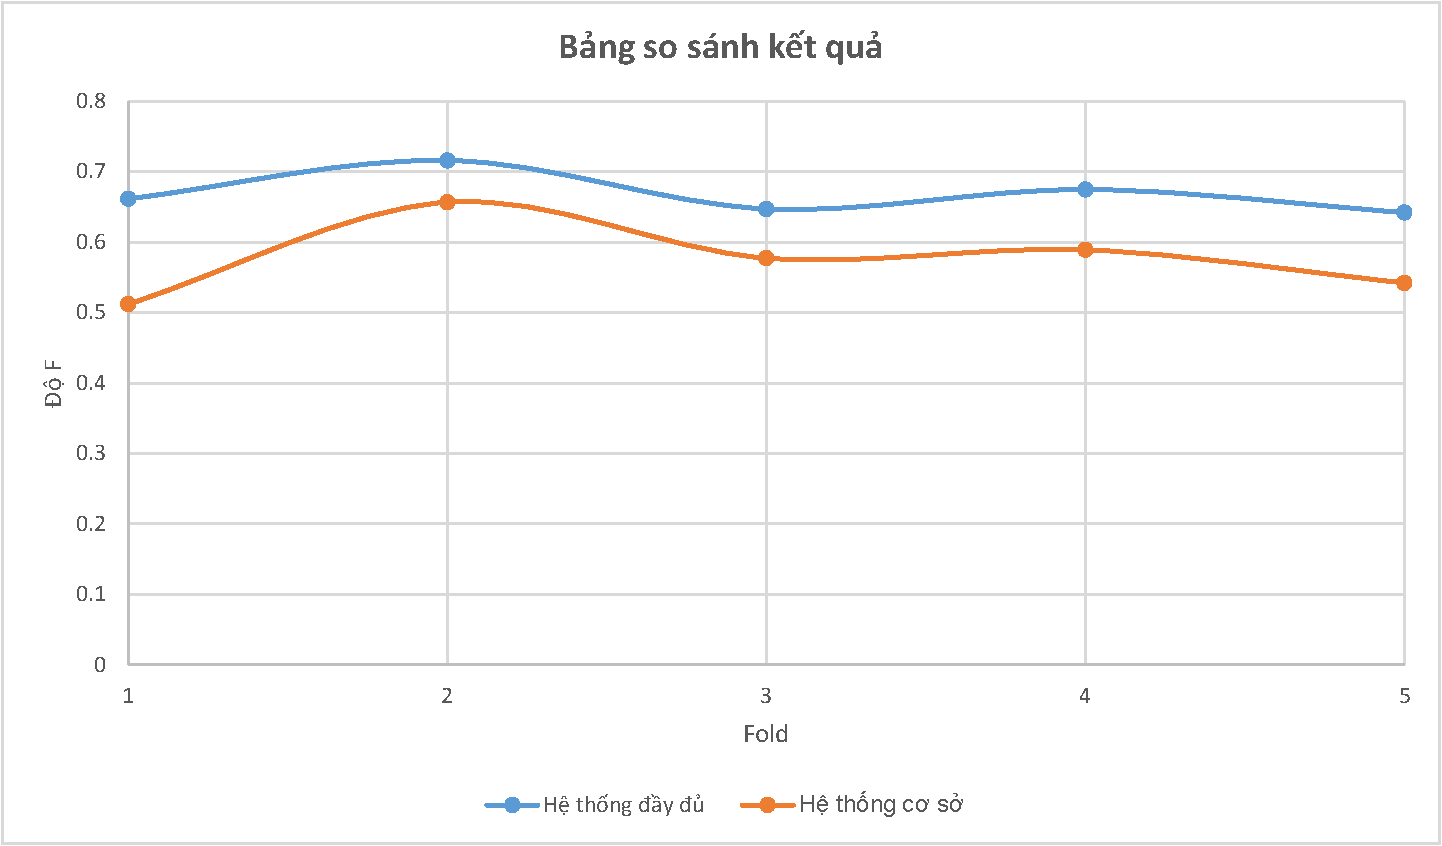
\includegraphics[scale=0.5]{charts/demo_chart.pdf}
					% 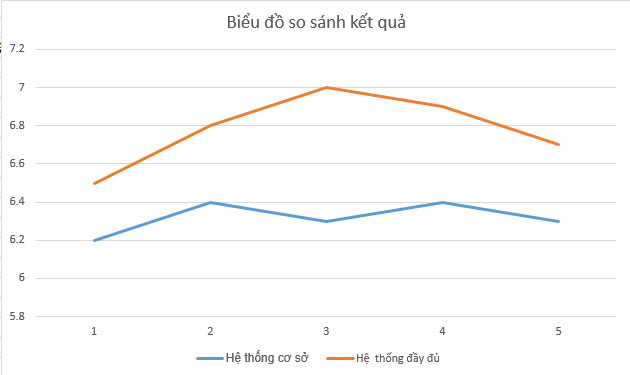
\includegraphics[width=\linewidth]{images/result.png}
					\caption{So sánh kết quả giữa hệ thống cơ sở và hệ thống đầy đủ}
				\end{figure} 

		\section{Phân tích kết quả thực nghiệm}
		\subsection*{Nhận xét}
		Dựa vào bảng kết quả 6.1, chúng tôi có một số nhận xét trực quan:
			\begin{itemize}
				\item{Hệ thống đầy đủ đạt kết quả cao hơn hệ thống cơ sở, cụ thể có độ F cao hơn khoảng ???\%. Điều này chứng tỏ các đặc trưng liên quan đến khai khoáng ý kiến đã ảnh hưởng tích cực đến kết quả, chúng có giá trị đối với bài toán đồng tham chiếu trên lĩnh vực khai khoáng ý kiến}.
				\item{Hệ thống SC đạt kết quả cao hơn hệ thống cơ sở khoảng ???\% độ F. Điều này cho thấy đặc trưng \textit{Tính nhất quán về ý kiến (SC)} đã có ảnh hưởng tương đối lớn đến hệ thống}.
				\item{Hệ thống SC+EOA đạt kết quả không cao hơn nhiều so với hệ thống SC, cao hơn khoảng ???\% độ F. Điều này cho thấy đặc trưng \textit{Sự kết hợp giữa thực thể và từ chỉ ý kiến (EOA)} đã có ảnh hưởng tiêu cực đến hệ thống, tuy nhiên vì một số lí do nào đó đặc trưng này tỏ ra không hiệu quả khi được sử dụng}.
			\end{itemize}
		\subsection*{Giải thích}
			\par Chúng tôi phân tích kết quả bằng cách đi trả lời hai câu hỏi: tại sao những đặc trưng liên quan đến khai khoáng ý kiến chưa đóng góp nhiều vào kết quả hệ thống và tại sao kết quả hệ thống chưa cao.
			\par \textit{Nguyên nhân đặc trưng \textit{Sự kết hợp giữa thực thể và từ chỉ ý kiến (EOA)} chưa ảnh hưởng nhiều đến hệ thống:}
				\begin{itemize}
					\item{Số lượng từ chỉ ý kiến trong tập dữ liệu vẫn chưa nhiều (chỉ có 442 trong số 2634 từ chỉ đối tượng, thuộc tính có từ chỉ ý kiến đi kèm). Do đó thuộc tính EOA vẫn chưa ảnh hưởng nhiều đến hệ thống}.
					\item{Các từ chỉ ý kiến trong tập dữ liệu vẫn chưa có tính đặc trưng cao, có những từ chỉ ý kiến có thể đi kèm với nhiều cụm danh từ khác nhau, ví dụ như tính từ \textit{“good”}, \textit{“nice”}, \textit{“better”}, \textit{“great”}. Trong câu \textit{“The M9 destroyed the Nexus 6 in both aspects. The battery life was pretty great. It wasn't as good as the Oneplus One, but was much better than the M9”}, khả năng từ \textit{“good”} liên kết được với \textit{“the M9”}, \textit{“Nexus 6”} và \textit{“the battery”} là tương đương nhau. Nên khó xác định được từ \textit{“It”} liên kết với \textit{“good”} đang chỉ đến cụm danh từ nào}.
					\item{Theo giả thuyết cặp nào có giá trị thuộc tính EOA càng nhỏ thì càng có khả năng đồng tham chiếu. Tuy nhiên trên thực tế có những cặp có giá trị thuộc tính EOA nhỏ (0 hoặc 1) nhưng không đồng tham chiếu, trong khi có nhiều cặp có giá trị EOA lớn (3 hoặc 4) thì cặp đó lại đồng tham chiếu}.
					\item{Tập dữ liệu học của thuộc tính EOA bị nhiễu. Một cụm danh từ có từ chỉ ý kiến nhưng trên thực tế nằm trong chuỗi đồng tham chiếu nào sẽ tạo ra các mẫu học có  giá trị thuộc tính EOA là 0,1,2,3,4, dẫn đến hệ thống học được rằng dù thuộc tính EOA là 0 hoặc 1 thì vẫn phân loại là không đồng tham chiếu. Chúng tôi thống kê thấy có 57 cụm danh từ có dạng như vậy}.
				\end{itemize}
			\par \textit{Nguyên nhân đặc trưng \textit{Tính nhất quán về ý kiến (SC)} chưa ảnh hưởng nhiều đến hệ thống}:
				\begin{itemize}
					\item{Giải thuật tìm thiên hướng ý kiến gắn với đối tượng/thuộc tính được nêu ra trong câu vẫn còn đơn giản và chỉ cho kết quả đúng đối với các câu tương đối đơn giản. Đối với dữ liệu thực tế mà minh chứng là dữ liệu do chúng tôi thu thập, có một số lượng nhất định các câu phức và việc xác định thiên hướng ý kiến này chưa cho hiệu quả cao.}					
				\end{itemize}
			\par \textit{Nguyên nhân hệ thống vẫn chưa đạt kết quả cao}:
				\begin{itemize}
					\item{Trong lĩnh vực khai khoáng ý kiến, có những trường hợp đồng tham chiếu chỉ có thể phát hiện được nhờ vào hai đặc trưng cơ bản liên quan đến khai khoáng ý kiến (\textit{Sự kết hợp giữa thực thể và từ chỉ ý kiến} và \textit{Tính nhất quán về ý kiến}). Tuy nhiên, vì một số lí do chúng tôi đã trình phần trên, hai đặc trưng đó vẫn chưa có nhiều ảnh hưởng đến hệ thống}.
					\item{Có những trường hợp một đối tượng được diễn tả bởi nhiều tên gọi khác nhau mà không đặc trưng nào trong hệ thống phát hiện ra được. Ví dụ: Để chỉ đối tượng là chiếc điện thoại Samsung Galaxy S3, có thể viết là \textit{"the GS3"} hoặc \textit{"the Samsung S3"} hoặc \textit{a new S3 SGH-I747 (US model) ATT phone}}.
					\item{}
				\end{itemize}

		
	\chapter{Tổng kết}	
		\section*{Kết quả đạt được}		
		\par Trong giai đoạn Luận văn tốt nghiệp, chúng tôi đã thực hiện được những công việc sau:
		\begin{itemize}
			\item{Giới thiệu bài toán Phân giải đồng tham chiếu và tìm hiểu về các công trình liên quan đến đồng tham chiếu nói chung.}
			\item{Tìm hiểu về các công trình liên quan đến đồng tham chiếu cho một số loại văn bản cụ thể.}
			\item{Tìm hiểu về các phương pháp Khai khoáng ý kiến và một số vấn đề trong Khai khoáng ý kiến.}
			\item{Giới thiệu bài toán Phân giải đồng tham chiếu cho đối tượng và thuộc tính trong Khai khoáng ý kiến, mô hình hóa bài toán và đề ra phương pháp giải quyết.}
			\item{Xây dựng hệ thống giải quyết bài toán dựa trên phương pháp đề xuất, cho kết quả đầu ra khả quan.}
		\end{itemize}
		\section*{Khó khăn và hạn chế}		
			\begin{itemize}
				\item{Chúng tôi có liên lạc với các tác giả Ding, Liu của bài báo \cite{mainpaper} và được biết dữ liệu mà họ thu thập và gán nhãn đã bị mất bởi một vài sự cố đáng tiếc. Do vậy chúng tôi đã tự thu thập và gán nhãn cho tập dữ liệu. Những dữ liệu này tuy đáp ứng được các yêu cầu của đề tài nhưng trong nhiều trường hợp, sự tồn tại của các câu phức tạp đã gây khó khăn cho hệ thống của chúng tôi, đặc biệt trong việc xác định các câu so sánh hay xác định thiên hướng ý kiến đối với các thực thể, làm ảnh hưởng đến kết quả thực nghiệm.}
				\item{Do những hạn chế về thời gian, chúng tôi không thể áp dụng và triển khai hệ thống phân giải đồng tham chiếu cho tiếng Việt. Chúng tôi chỉ kịp khảo sát các trang mạng có chứa văn bản ý kiến trong tiếng Việt và thử một số công cụ xử lý ngôn ngữ tiếng Việt như JVNTextPro, VietChunker hay VnDP.}
			\end{itemize}	
		\section*{Hướng phát triển của đề tài}		
		\begin{itemize}
			\item{Trong tương lai, có thể tìm thêm những đặc trưng liên quan đến Khai khoáng ý kiến khác để áp dụng vào hệ thống nhằm tăng độ chính xác.}
			\item{Cải tiến, mở rộng đặc trưng \textit{Sự kết hợp giữa thực thể và từ chỉ ý kiến}. Hiện tại, chúng tôi chỉ mới sử dụng từ chỉ ý kiến là tính từ và trạng từ. Chúng tôi đề xuất sử dụng thêm những từ chỉ ý kiến là danh từ như “problem” và bổ sung thêm danh sách những từ không chỉ ý kiến nhưng chúng thường đi kèm với một vài thuộc tính nhất định; nói cách khác, quan hệ giữa chúng với các đối tượng, thuộc tính khác nhau là khác nhau.}
			\item{Thử nghiệm cho tiếng Việt:
				\begin{itemize}
					\item{Các văn bản chứa ý kiến trong tiếng Việt có thể là các bài đánh giá (review) trên Tiki hay các bài thảo luận (discussion) trên tinhte.vn, ...
					}
					\item{Hiện nay đã có các công cụ Xử lý ngôn ngữ tự nhiên dùng cho tiếng Việt. Dưới đây chúng tôi sẽ trình bày về ba công cụ JVnTextPro (tách câu, tách từ, gán nhãn từ loại), VietChunker(gom cụm từ) và VnDP(phân tích văn phạm phụ thuộc), chúng có thể được sử dụng cho hệ thống phân giải đồng tham chiếu trong tiếng Việt (tương tự như hệ thống dùng cho tiếng Anh).					
					\\Công cụ JVnTextPro \footnote{http://jvntextpro.sourceforge.net} là công cụ có thể được dùng để phân đoạn câu (sentence segmentation), phân đoạn thẻ câu (sentence tokenization), phân đoạn từ (word tokenization) và gán nhãn từ loại (POS tagging) cho văn bản tiếng Việt.
					\\Ví dụ: Cho đoạn văn bản tiếng Việt sau (Lấy trên trang Tiki.vn)
					\\\textit{iPhone 6S đã chính thức được ra mắt với thiết kế không khác biệt so với iPhone 6. Điểm khác biệt về ngoại hình là bộ đôi Phone 6s và 6s Plus sẽ có tới 4 màu sắc bao gồm: xám, bạc, vàng và vàng hồng, và có thêm chữ "S" phía sau mặt lưng. iPhone 6s sẽ nặng hơn iPhone 6 14g, iPhone 6s dài, dày, rộng hơn iPhone 6 chút ít, nhưng người ta khó nhận ra bằng mắt thường bởi con số này chỉ tính là một vài mm, thậm chí chưa đến 1 mm.}
					\\Dưới đây là kết quả đầu ra sau khi xử lý văn bản trên bằng JVnTextPro:
					\begin{figure}[H]
						\centering				
						\noindent\fbox{
						    \parbox{\textwidth}{
						        iPhone/X 6S/M đã/R chính\_thức/A được/V ra\_mắt/V với/C thiết\_kế/V không/R khác\_biệt/A so/V với/E iPhone/T 6./M Điểm/N khác\_biệt/A về/E ngoại\_hình/N là/C bộ/Nc đôi/M Phone/N 6s/M và/C 6s/M Plus/Np sẽ/R có/V tới/T 4/M màu\_sắc/N bao\_gồm/V :/: xám/A ,/, bạc/N ,/, vàng/Np và/C vàng/A hồng/A ,/, và/C có/V thêm/V chữ/N S/M phía/N sau/N mặt\_lưng/N ./.
						        \\
						        \\
								iPhone/N 6s/M sẽ/R nặng/A hơn/A iPhone/N 6/M 14g/Nu ,/, iPhone/N 6s/M dài/A ,/, dày/A ,/, rộng/A hơn/A iPhone/N 6/M chút\_ít/N ,/, nhưng/C người\_ta/N khó/A nhận\_ra/X bằng/E mắt\_thường/A bởi/E con\_số/N này/Np chỉ/R tính/Ny là/C một\_vài/N mm/N ,/, thậm\_chí/R chưa/R đến/V 1/M mm/N ./.
					    	}
						}
						\caption{Ví dụ gán nhãn từ loại cho văn bản tiếng Việt bằng công cụ JVnTextPro}
					\end{figure}
					VnDP \footnote{https://sourceforge.net/projects/vndp/files/VnDPv1.0.1.zip} là công cụ dùng cho phân tích văn phạm phụ thuộc trong tiếng Việt. Có thể xem một ví dụ phân tích văn phạm phụ thuộc cho câu "iPhone 6s sẽ nặng hơn iPhone 6 14g, iPhone 6s dài, dày, rộng hơn iPhone 6 chút ít, nhưng người ta khó nhận ra bằng mắt thường bởi con số này chỉ tính là một vài mm, thậm chí chưa đến 1 mm." như sau:	
					\begin{table}[H]
						\centering													
						\begin{tabular}{ | l | l | l | l | l | l | l | l | l | l | }
\hline
	1 & iPhone & iPhone & N & N & - & 4 & sub & - & - \\ \hline
	2 & 6s & 6s & M & M & - & 1 & det & - & - \\ \hline
	3 & sẽ & sẽ & R & R & - & 4 & amod & - & - \\ \hline
	4 & nặng & nặng & A & A & - & 0 & root & - & - \\ \hline
	5 & hơn & hơn & A & A & - & 4 & amod & - & - \\ \hline
	6 & iPhone & iPhone & N & N & - & 4 & dob & - & - \\ \hline
	7 & <num> & <num> & M & M & - & 6 & det & - & - \\ \hline
	8 & 14g, & 14g, & M & M & - & 9 & det & - & - \\ \hline
	9 & iPhone & iPhone & N & N & - & 6 & nmod & - & - \\ \hline
	10 & 6s & 6s & M & M & - & 11 & det & - & - \\ \hline
	11 & dài, & dài, & N & N & - & 9 & nmod & - & - \\ \hline
	12 & dày, & dày, & N & N & - & 11 & nmod & - & - \\ \hline
	13 & rộng & rộng & A & A & - & 11 & nmod & - & - \\ \hline
	14 & hơn & hơn & A & A & - & 13 & amod & - & - \\ \hline
	15 & iPhone & iPhone & N & N & - & 13 & amod & - & - \\ \hline
	16 & <num> & <num> & M & M & - & 15 & det & - & - \\ \hline
	17 & chút & chút & L & L & - & 18 & det & - & - \\ \hline
	18 & ít, & ít, & N & N & - & 15 & nmod & - & - \\ \hline
	19 & nhưng & nhưng & C & C & - & 18 & coord & - & - \\ \hline
	20 & người & người & N & N & - & 23 & sub & - & - \\ \hline
	21 & ta & ta & P & P & - & 20 & nmod & - & - \\ \hline
	22 & khó & khó & A & A & - & 23 & vmod & - & - \\ \hline
	23 & nhận & nhận & V & V & - & 19 & conj & - & - \\ \hline
	24 & ra & ra & R & R & - & 23 & adv & - & - \\ \hline
	25 & bằng & bằng & E & E & - & 23 & mnr & - & - \\ \hline
	26 & mắt & mắt & N & N & - & 25 & pob & - & - \\ \hline
	27 & thường & thường & R & R & - & 23 & adv & - & - \\ \hline
	28 & bởi & bởi & E & E & - & 23 & prp & - & - \\ \hline
	29 & con & con & N & N & - & 33 & sub & - & - \\ \hline
	30 & số & số & N & N & - & 29 & nmod & - & - \\ \hline
	31 & này & này & P & P & - & 29 & det & - & - \\ \hline
	32 & chỉ & chỉ & R & R & - & 33 & adv & - & - \\ \hline
	33 & tính & tính & V & V & - & 28 & dep & - & - \\ \hline
	34 & là & là & V & V & - & 33 & vmod & - & - \\ \hline
	35 & một & một & M & M & - & 37 & det & - & - \\ \hline
	36 & vài & vài & L & L & - & 37 & det & - & - \\ \hline
	37 & mm, & mm, & N & N & - & 33 & dob & - & - \\ \hline
	38 & thậm & thậm & N & N & - & 37 & nmod & - & - \\ \hline
	39 & chí & chí & N & N & - & 38 & nmod & - & - \\ \hline
	40 & chưa & chưa & R & R & - & 41 & adv & - & - \\ \hline
	41 & đến & đến & V & V & - & 33 & tmp & - & - \\ \hline
	42 & <num> & <num> & M & M & - & 43 & det & - & - \\ \hline
	43 & mm. & mm. & N & N & - & 41 & dob & - & - \\ \hline
\end{tabular}

						\caption{Ví dụ phân tích văn phạm phụ thuộc cho tiếng Việt bằng công cụ VnDP}
					\end{table}	
					Dựa trên kết quả gán nhãn từ loại bằng công cụ JVnTextPro, có thể gom các cụm danh từ nhờ vào công cụ VietChunker \footnote{http://vlsp.hpda.vn:8080/demo/?page=resources\&tool=chunker}.	
					}					
					\item{Các nghiên cứu liên quan đến Phân giải đồng tham chiếu và Khai khoáng ý kiến trong tiếng Việt cũng đã xuất hiện trong những năm gần đây. (Lê Đức Trọng, 2011) trong \cite{leductrong11} đã áp dụng mô hình học máy có giám sát SVM trên dữ liệu thu thập từ vnexpress.net, mô hình phân giải đồng tham chiếu của tác giả trên dữ liệu này cho độ chính xác 76.51\%. Trong \cite{vn_sentiment1} và \cite{vn_sentiment2}, các tác giả cũng đã đưa ra mô hình Khai khoáng ý kiến cho văn bản tiếng Việt.}
				\end{itemize}
				Những công cụ và công trình này là gợi ý để có thể áp dụng mô hình phân giải đồng tham chiếu của chúng tôi cho tiếng Việt.
			}
		\end{itemize}
\renewcommand{\refname}{Tham khảo} 

%----------REFERENCES-------------------
\newpage
\addcontentsline{toc}{chapter}{Tham khảo}
\begin{thebibliography}{30}

	\bibitem{mainpaper} 
	Xiaowen Ding and Bing Liu. 2010.
	\textit{Resolving Object and Attribute Coreference in Opinion Mining}. 
	In Proceedings of International Conference on Computational Linguistics (COLING-2010). 2010.
	 
	\bibitem{findfeatures1} 
	Minqing Hu and Bing Liu. 2004.
	\textit{Mining and Summarizing Customer Reviews}.
	In Proceedings of the ACM SIGKDD International Conference on Knowledge Discovery and Data Mining (KDD-2004), Aug 22-25, 2004, Seattle, Washington, USA.

	\bibitem{findfeatures2} 
	A-M. Popescu and O. Etzioni. 2005. 
	\textit{Extracting product features and opinions from reviews}.
	EMNLP’05.

	\bibitem{corefdef}
	Joseph F. Mccarthy. 1996.
 	\textit{A trainable approach to coreference resolution for information extraction}.

 	\bibitem{sentiment}
 	Bing Liu. 2010.
 	\textit{Sentiment Analysis and Subjectivity}. A chapter in 
  	Handbook of Natural Language Processing, Second Edition, 
  	(editors: N. Indurkhya and F. J. Damerau), 2010.

  	\bibitem{comparative1}
  	Nitin Jindal and Bing Liu. 2006.  
  	\textit{Identifying Comparative Sentences in Text Documents}. 
   	In Proceedings of the ACM SIGIR International Conference on 
   	Information Retreival (SIGIR-06), 2006.

   	\bibitem{comparative2}
	G. Ganapathibhotla and B. Liu. 2008.
	\textit{Identifying Preferred Entities in Comparative Sentences}.
	In Proceedings of the International Conference on Computational Linguistics, COLING, 2008.

	\bibitem{mltextbook}
	Tom Mitchell, McGraw Hill, 1997.
	\textit{Machine Learning}.
	Publisher: McGraw-Hill Science/Engineering/Math; (March 1, 1997). ISBN-0070428077.	

	\bibitem{crfchunker}
	Xuan-Hieu Phan. 2006.
	\textit{CRFChunker: CRF English Phrase Chunker}. 
	http://crfchunker.sourceforge.net/.

	\bibitem{ng02}
	Vincent Ng and Claire Cardie. 2002.
	\textit{Improving Machine Learning Approaches to Coreference Resolution}.
	In Proceedings of the 40th Annual Meeting of the Association for Computational Linguistics, pages 104–111.

	\bibitem{dagan90}
	Ido Dagan and Alon Itai. 1990.
	\textit{Automatic processing of large corpora for the resolution of anaphora references}.
	In Proceedings of the 13th International Conference on Computational Linguistics, pages 330–332.

	\bibitem{kehler04}
	Andrew Kehler, Douglas Appelt, Lara Taylor, and Aleksandr Simma. 2004.
	\textit{Competitive self-trained pronoun interpretation}.
	In Proceedings of the Human Language Technologies and North American Association for Computational Linguistics 2004: Short Papers, pages 33–36.

	\bibitem{yang05}
	Xiaofeng Yang, Jian Su, and Chew Lim Tan. 2005.
	\textit{Improving pronoun resolution using statistics-based semantic compatibility information}.
	In Proceedings of the 43rd Annual Meeting of the Association for Computational Linguistics, pages 165–172.

	\bibitem{haghighi09}
	Aria Haghighi and Dan Klein. 2009.
	\textit{Simple coreference resolution with rich syntactic and semantic features}.
	In Proceedings of the 2009 Conference on Empirical Methods in Natural Language Processing, pages 1152–1161.

	\bibitem{soon01}
	Wee Meng Soon, Hwee Tou Ng, and Daniel Chung Yong Lim. 2001.
	\textit{A machine learning approach to coreference resolution of noun phrases}.
	Computational Linguistics, 27(4):521–544.

	\bibitem{mccallum04}
	Andrew McCallum and Ben Wellner. 2004.
	\textit{Conditional models of identity uncertainty with application to noun coreference}.
	In Advances in Neural Information Proceesing Systems.

	\bibitem{lou04}
	Xiaoqiang Luo, Abe Ittycheriah, Hongyan Jing, Nanda Kambhatla and Salim Roukos. 2004.
	\textit{A Mention-Synchronous Coreference Resolution Algorithm Based On the Bell Tree}.
	In Proceedings of the 42nd Meeting of the Association for Computational Linguistics (ACL'04), Main Volume.

	\bibitem{yang04}
	Xiaofeng Yang, Jian Su, GuoDong Zhou, and Chew Lim Tan. 2004.
	\textit{An NP-cluster based approach to coreference resolution}.
	In Proceedings of the 20th International Conference on Computational Linguistics, pages 226–232.

	\bibitem{yang08}
	Xiaofeng Yang, Jian Su, Jun Lang, Chew Lim Tan and Sheng Li. 2008.
	\textit{An entity-mention model for coreference resolution with inductive logic programming}.
	In Proceedings of the 46th Annual Meeting of the Association for Computational Linguistics: Human Language Technologies, pages 843–851.

	\bibitem{culotta07}
	Aron Culotta, Michael Wick, Robert Hall and Andrew McCallum. 2007.
	\textit{First-Order Probabilistic Models for Coreference Resolution}.
	In Proceedings of Human Language Technologies 2007.

	\bibitem{connolly95}
	Dennis Connolly, John D. Burger, and David S. Day. 1994.
	\textit{A machine learning approach to anaphoric reference}.
	In Proceedings of International Conference on New Methods in Language Processing, pages 255–261.

	\bibitem{connolly97}
	Dennis Connolly, John D. Burger, and David S. Day. 1997.
	\textit{A machine learning approach to anaphoric reference}.
	In D. Jones and H. Somers, editors, New Methods in Language Processing, pages 133–144. UCL Press.

	\bibitem{iida03}
	Ryu Iida, Kentaro Inui, Hiroya Takamura, and Yuji Matsumoto. 2003.
	\textit{Incorporating contextual cues in trainable models for coreference resolution}.
	In Proceedings of the EACL Workshop on The Computational Treatment of Anaphora.

	\bibitem{yang03}
	Xiaofeng Yang, Guodong Zhou, Jian Su, and Chew Lim Tan. 2003.
	\textit{Coreference resolution using competitive learning approach}.
	In Proceedings of the 41st Annual Meeting of the Association for Computational Linguistics, pages 176–183.

	\bibitem{denis08}
	Pascal Denis and Jason Baldridge. 2008.
	\textit{Specialized models and ranking for coreference resolution}.
	In Proceedings of the 2008 Conference on Empirical Methods in Natural Language Processing, pages 660–669.

	\bibitem{rahman09}
	Altaf Rahman and Vincent Ng. 2009.
	\textit{Supervised models for coreference resolution}.
	In Proceedings of the 2009 Conference on Empirical Methods in Natural Language Processing, pages 968–977.

	\bibitem{yang06}
	Xiaofeng Yang, Jian Su, and Chew Lim Tan. 2006.
	\textit{Kernel based pronoun resolution with structured syntactic knowledge}.
	In Proceedings of the 21st International Conference on Computational Linguistics and the 44th Annual Meeting of the Association
	for Computational Linguistics, pages 41–48.

	\bibitem{ng08}
	Vincent Ng. 2008.
	\textit{Unsupervised models for coreference resolution}.
	In Proceedings of the 2008 Conference on Empirical Methods in Natural Language Processing, pages 640–649.

	\bibitem{poon08}
	Hoifung Poon and Pedro Domingos. 2008.
	\textit{Joint unsupervised coreference resolution with Markov Logic}.
	In Proceedings of the 2008 Conference on Empirical Methods in Natural Language Processing, pages 650–659.

	\bibitem{baldwin95}
	Frederick Breckenridge Baldwin. 1995.
	\textit{CogNiac: A Discourse Processing Engine}.
	PhD thesis, University of Pennsylvania Department of Computer and Information Science, 1995.

	\bibitem{brown93}
	Peter F. Brown and Stephen A. Della Pietra and Vincent J. Della Pietra and Robert. L. Mercer. 1993.
	\textit{The mathematics of statistical machine translation: parameter estimation}.
	In the Computational Linguistics,  Vol. 19, pages 263-311.

	\bibitem{collin99}
	Collins, Michael and Yoram Singer. 1999.
	\textit{Unsupervised models for named entity classification}.
	In Proceedings of the 2000 Joint SIGDAT Conference on Empirical Methods in Natural Language Processing and Very Large Corpora, pages 100–110.

	\bibitem{spitkovsky10}
	Spitkovsky, Valentin I., Hiyan Alshawi and Daniel Jurafsky. 2010.
	\textit{From baby steps to leapfrog: How "less is more" in unsupervised dependency parsing}.
	In Human Language Technologies: The 2010 Annual Conference of the North American Chapter of the Association for Computational Linguistics, pages 751–759.

	\bibitem{lee12}
	Heeyoung Lee, Angel Chang, Yves Peirsman, Nathanael Chambers, Mihai Surdeanu and Dan Jurafsky. 2012.
	\textit{Deterministic Coreference Resolution Based on Entity-Centric, Precision-Ranked Rules}.
	In the Computational Linguistics,  Vol. 39, No.4, pages 885-916.

	\bibitem{li15}
	Qiang Li, Zongtian Liu, Lei Chen and Xianchuan Wang. 2015.
	\textit{An Event-Oriented Multi-pass Sieve Module for Coreference Resolution}.
	Published in: Intelligent Systems and Knowledge Engineering (ISKE), 2015 10th International Conference.

	\bibitem{stoyanov06}
	Veselin Stoyanov and Claire Cardie. 2006.
	\textit{Partially supervised coreference resolution for opinion summarization through structured rule learning}.
	In Proceedings of the 2006 Conference on Empirical Methods in Natural Language
	Processing (EMNLP), pages 336-344.

	\bibitem{nicolov08}
	N. Nicolov, F. Salvetti and S. Ivanova. 2008.
	\textit{Sentiment analysis: Does coreference matter?}.
	In AISB 2008 Convention Communication, Interaction and Social Intelligence.	

	\bibitem{weiss03}
	Weiss, G. and Provost,F. 2003.
	\textit{Learning when Training Data are Costly: The Effect of Class Distribution on Tree Induction}.
	Journal of ArtiJicial Intelligence Research, Vol:19, pages 315-354.

	\bibitem{leductrong11}	
	Duc-Trong Le, Mai-Vu Tran, Tri-Thanh Nguyen, Quang-Thuy Ha. 2011.
	\textit{Co-reference Resolution in Vietnamese Documents Based on Support Vector Machines}.
	IALP 2011: 89-93, Penang, Malaysia.

	\bibitem{vn_sentiment1}
	Binh Thanh Kieu, Son Bao Pham. 2010.
	\textit{Sentiment Analysis for Vietnamese}.
	International Conference on Knowledge and Systems Engineering: IEEE CS, 2010.

	\bibitem{vn_sentiment2}
	Quang-Thuy Ha, Tien-Thanh Vu, Huyen-Trang Pham, Cong-To Luu. 2011.
	\textit{An Upgrading Feature-based Opinion Mining Model on Product Reviews in Vietnamese}.
	AMT’2011: 173-185, Lanzhou, China.

	\bibitem{vilain95}
	Vilain, Marc, John Burger, John Aberdeen, Dennis Connolly and Lynette Hirschman. 1995.
	\textit{A model-theoretic coreference scoring scheme}.
	In Proceedings of the 6th Message Understanding Conference (MUC-6), pages 45–52.

	\bibitem{bagga98}
	Amit Bagga and Breck Baldwin. 1998.
	\textit{Algorithms for Scoring Coreference Chains}.
	In The First International Conference on Language Resources and Evaluation Workshop on Linguistics Coreference.

	\bibitem{lou05}
	Xiaoqiang Luo. 2005.
	\textit{On coreference resolution performance metrics}.
	In Proceedings of the Human Language Technology Conference and the 2005 Conference on Empirical Methods in Natural Language Processing, Vancouver, B.C., Canada, 6–8 October 2005, pages 25–32
 
\end{thebibliography}	

\end{document}
